\documentclass[conference]{IEEEtran}
\IEEEoverridecommandlockouts
\usepackage{cite}
\usepackage{amsmath,amssymb,amsfonts}
\usepackage{graphicx}
\usepackage{textcomp}
\usepackage{xcolor}
\usepackage{booktabs}
\usepackage{array}
\usepackage{adjustbox}
\usepackage{url}
\usepackage[hidelinks]{hyperref}
\graphicspath{{figures/}}

\newcommand{\sat}{\mathrm{sat}}
\newcommand{\Proj}{\mathrm{Proj}}

% 表格自然宽度实测：把每个 tabular 的宽度写进 .log，供 measure_tables.py 解析，
% 从而用【实测值】而不是估算值决定这张表能否放进单栏。
\newsavebox{\wigmeasurebox}
\newcommand{\wigmeasure}[2]{%
  \sbox{\wigmeasurebox}{#2}%
  \typeout{WIGTABLEWIDTH #1 = \the\wd\wigmeasurebox}%
  \usebox{\wigmeasurebox}}

% 浮动体间距：IEEEtran 默认约 12 pt，本文图表较多，收紧到 6 pt 以节省版面，
% 不影响可读性，也不改变 IEEE 的字体与栏宽规范。
\setlength{\textfloatsep}{4pt plus 2pt minus 2pt}
\setlength{\floatsep}{4pt plus 2pt minus 2pt}
\setlength{\intextsep}{4pt plus 2pt minus 2pt}

\begin{document}

\title{RBF Neural-Network Adaptive Longitudinal Flight Control of a Wing-in-Ground-Effect UAV: Height-Instability Mechanism and Simulation Validation}

\author{
\IEEEauthorblockN{}
}

\maketitle

\begin{abstract}
Small wing-in-ground-effect (WIG) vehicles operate entirely inside the strong ground-effect regime, where the aerodynamics vary sharply with height and the longitudinal dynamics exhibit two stability problems absent in conventional aircraft. This paper studies a WIG UAV of 2.40 m span and 12.0 kg mass cruising at 18 m/s at heights between 0.05 m and 0.50 m. A seventh-order nonlinear longitudinal model with a ground-effect correction is established. Two results are established quantitatively. First, the pitch-moment height derivative is strictly positive throughout the envelope, from +1.06 to +14.90 N$\cdot$m/m, so the height static stability is negative; a component-wise decomposition shows that the tail downwash term dominates (+15.78 N$\cdot$m/m) while the wing provides a stabilising contribution (-2.30 N$\cdot$m/m). Second, the phugoid-height coupled mode becomes unstable, with real part up to +0.4875 1/s, whereas switching the ground effect off returns the mode to neutral stability, proving that the instability is of ground-effect origin. A three-loop controller is then designed, comprising an altitude outer loop, a dynamic-surface attitude inner loop and an airspeed loop, with two RBF networks and tanh robust terms acting in the moment and drag channels. Closed-loop uniform ultimate boundedness is proved by a Lyapunov argument. A discrete-time design constraint, $T_s\Gamma_i\|\phi_i\|^2 < k_i$, is further derived; it explains why the moment-channel adaptation gain must be three orders of magnitude smaller than the drag-channel gain. Simulations with significant ground-effect mismatch, RAM effect and lift nonlinearity show that the height-tracking RMS error is reduced from 0.1938 m to 0.0100 m (a factor of 19.4), the Monte-Carlo pass rate rises from 40.0\% to 86.7\%, and safe flight is maintained at an extreme altitude of 0.06 m, under measurement noise and in moderate gusts.
\end{abstract}

\begin{IEEEkeywords}
wing-in-ground effect; flight control; RBF neural network; adaptive control; dynamic surface control; height stability
\end{IEEEkeywords}

\section{Introduction}
A wing-in-ground-effect (WIG) vehicle exploits the suppression of downwash by the ground image vortex system when flying close to the ground or sea surface, obtaining a substantially increased lift-curve slope and a sharply reduced induced drag, and hence a lift-to-drag ratio far above that of a conventional aircraft [1], [2]. Small WIG unmanned aerial vehicles have a short span and a low cruising height, so their entire operating envelope lies inside the strong ground-effect regime. For the configuration studied here, at $h = 0.05$ m the induced drag is only 5.1\% of its free-air value and the lift-curve slope is 34.3\% higher; even at $h = 0.50$ m the lift-curve slope is still 11.7\% higher. This height-dependent aerodynamics makes the flight control problem fundamentally different from that of a conventional aircraft.

The difficulty concentrates in two points. The first is negative height static stability. As early as the 1970s Irodov pointed out that the height-stability criterion for a WIG vehicle requires $\partial C_m/\partial h < 0$, which most WIG configurations do not satisfy [3]. The decomposition given in Section III shows that for the present configuration $\partial M/\partial h = +1.06$ to +14.90 N$\cdot$m/m over the whole envelope. The second is the instability of the phugoid-height coupled mode: the ground effect turns the classically neutrally stable phugoid mode into an unstable one, with the real part of the low-frequency mode reaching +0.4875 1/s. Together these two facts make an actively controlled altitude loop with sufficient bandwidth mandatory [5], [6], [18]-[21], [23], [24].

\subsection{Related Work}
For aerodynamic modelling, quasi-steady ground effect is usually represented by a downwash-retention factor that measures how strongly the image vortex system suppresses the downwash, and which then corrects the induced drag and the effective lift-curve slope [1], [6]. Wind-tunnel and CFD studies agree that ground effect raises the lift-curve slope and lowers the induced drag substantially, and that it shifts the height focus, thereby degrading longitudinal static stability; the stability criteria for a WIG vehicle therefore differ from those of a conventional aircraft and must be satisfied for both the angle-of-attack focus and the height focus [3]-[5], [18]-[21], [23], [24]. On the control side, RBF neural networks are widely used for direct adaptive control of uncertain nonlinear systems because of their universal approximation property and linearly parameterised weights; the Lyapunov framework was established by Sanner and Slotine [7], by Polycarpou [8] and by Ge and Wang [14]. Robust terms commonly use a tanh saturation function to smooth the sign function, a smoothing idea that is widespread in robust adaptive design [9], [10]; the projection operator used to guarantee uniformly bounded weights is due to Ioannou and Sun [10]. For backstepping implementations, dynamic surface control (DSC) and command-filtered backstepping avoid the analytic differentiation of virtual controls through first- or second-order filters, removing the "explosion of terms" [11]-[13]. The framework has recently been extended to the longitudinal control of vehicles with wide flight envelopes [22], [26].

However, most published work on adaptive control of WIG vehicles, including active-disturbance-rejection and stability-augmentation designs [25], validates the design against the nominal plant and rarely discusses the stability constraint that appears when an RBF adaptation law designed in continuous time is implemented digitally. That continuous-time adaptation laws can lose robustness in the presence of unmodelled dynamics was demonstrated long ago by the Rohrs counterexample [15], and discrete-time adaptive control has its own Lyapunov synthesis [16], [17]. The present work addresses exactly these two points.

\subsection{Contributions}
Taking a small WIG UAV as the plant, this paper makes the following contributions:

\begin{enumerate}
  \item a seventh-order nonlinear longitudinal model with ground-effect correction is established, in which the nominal/true mismatch (ground-effect strength, RAM effect and lift nonlinearity) is constructed explicitly so that the quantity the adaptive controller must compensate is measurable;
  \item a component-wise decomposition of the pitch-moment height derivative $\partial M/\partial h$ is given, proving quantitatively that the tail downwash term dominates the height instability while the wing term is stabilising, together with the height dependence of every term;
  \item it is proved quantitatively that the phugoid-height coupled mode instability originates entirely from the ground effect: switching the ground effect off returns the mode to neutral stability;
  \item a three-loop adaptive controller is designed with RBF networks and tanh robust terms in the moment and drag channels, and closed-loop uniform ultimate boundedness (UUB) is proved by a Lyapunov argument;
  \item the discrete-time stability criterion $T_s\Gamma_i\|\phi_i\|^2 < k_i$ is derived, which explains, from both dimensional scaling and sampling, why the two channel gains differ by three orders of magnitude;
  \item the design is validated by ablation, parameter perturbation, atmospheric disturbance, extreme low-altitude flight and Monte-Carlo statistics, and cross-checked between a Simulink model and a pure MATLAB script.
\end{enumerate}

\subsection{Principal Results}
\begin{table}[!t]
\centering
\caption{Performance of the three control schemes (true plant with ground-effect mismatch, RAM effect and lift nonlinearity)}
\label{tab:perf}
\footnotesize
\setlength{\tabcolsep}{4pt}
\begin{adjustbox}{max width=\columnwidth}
\wigmeasure{perf}{%
\begin{tabular}{lccc}
\toprule
Metric & RBF adaptive & DI + robust & Pure DI \\
\midrule
Height-tracking RMS error / m & 0.0100 & 0.1938 & 0.2119 \\
Peak height error / m & 0.0420 & 0.2500 & 0.2706 \\
Minimum height above ground / m & 0.1000 & 0.0000 & 0.0000 \\
Airspeed-tracking RMS error / (m/s) & 9.9000 & 3.9000 & 3.7000 \\
Monte-Carlo pass rate / \% & 86.7 & -- & 40.0 \\
Median height RMS error / m & 0.01040 & -- & 0.22322 \\
\bottomrule
\end{tabular}}
\end{adjustbox}
\end{table}

\section{Vehicle Model and Ground-Effect Aerodynamics}
\subsection{Configuration and Coordinate Frame}
A body-fixed frame is used ($x_b$ forward, $y_b$ to the right wing, $z_b$ towards the belly). The pitch rate $q$ and the pitch moment $M$ are positive nose-up. The main parameters are listed in Table II. The ground-effect flight band is $h = 0.05$ to $0.50$ m, corresponding to $h/b = 0.021$ to $0.208$. The following assumptions are made: (i) lateral-directional motion is neglected and the longitudinal motion is decoupled; (ii) the ground is a rigid plane and waves and roughness are ignored; (iii) the aerodynamics are quasi-steady and unsteady hysteresis is neglected; (iv) gusts are accounted for through the relative flow direction only, neglecting inertia terms due to the gust gradient.

\begin{table}[!t]
\centering
\caption{Main parameters of the reference configuration}
\label{tab:params}
\footnotesize
\setlength{\tabcolsep}{4pt}
\begin{adjustbox}{max width=\columnwidth}
\wigmeasure{params}{%
\begin{tabular}{lcclcc}
\toprule
Parameter & Symbol & Value & Parameter & Symbol & Value \\
\midrule
Wing span & $b$ & 2.40 m & Mass & $m$ & 12.0 kg \\
Chord & $c$ & 0.40 m & Pitch inertia & $I_{yy}$ & 1.15 kg$\cdot$m$^2$ \\
Wing area & $S$ & 0.96 m$^2$ & Max. thrust & $T_{\max}$ & 35 N \\
Aspect ratio & $AR$ & 6.0 & Cruise speed & $V_0$ & 18 m/s \\
Zero-lift angle & $\alpha_{L0}$ & $-3.0^{\circ}$ & Cruise height & $h_0$ & 0.20 m \\
Tail area & $S_t$ & 0.18 m$^2$ & Tail arm & $l_t$ & 0.95 m \\
Tail incidence & $i_t$ & $-2.0^{\circ}$ & Tail height offset & $\Delta z_t$ & 0.30 m \\
Elevator time const. & $\tau_e$ & 0.05 s & Engine time const. & $\tau_T$ & 0.15 s \\
\bottomrule
\end{tabular}}
\end{adjustbox}
\end{table}

\subsection{Ground-Effect Aerodynamic Model}
Let the ground-effect factor $\kappa(h)$ be the retention coefficient of the induced downwash: $\kappa = 1$ corresponds to free air and $\kappa \to 0$ to full ground contact. The following one-parameter family is adopted:

\begin{equation}
\adjustbox{max width=\columnwidth}{$\displaystyle \kappa(h) = \frac{x^{n}}{A + x^{n}}, \qquad x = \frac{h}{b}$}
\end{equation}

The shape parameters are $A = 0.0641$ and $n = 1.4622$. The expression is a physically motivated one-parameter family: it tends to zero as $h \to 0$ and to unity as $h \to \infty$, and the parameters were chosen so that the height dependence follows the monotonically increasing, saturating trend reported in the literature [1], [3], [4]. \textbf{It should be stated explicitly} that this paper does \textbf{not} claim the model has been quantitatively calibrated against wind-tunnel or CFD data for this configuration; such a calibration is future work (Section VI-A). What is studied here is whether the controller remains safe under a mismatch of this kind. Under ground effect the induced drag and the effective lift-curve slope become

\begin{equation}
\adjustbox{max width=\columnwidth}{$\displaystyle C_{Di}(h) = \frac{C_L^{2}\,\kappa(h)}{\pi\, AR\, e}, \qquad a_w(h) = \frac{a_0}{1 + a_0\,\kappa(h)/(\pi\, AR\, e)}$}
\end{equation}

The downwash angle at the tail is attenuated by the same factor, $\varepsilon(h,\alpha) = (\varepsilon_0 + \varepsilon_\alpha \alpha)\,\kappa(h)$. Fig. 1 shows the ground-effect factor, the lift-curve-slope gain and the induced drag as functions of height.

\begin{figure}[!t]
\centering
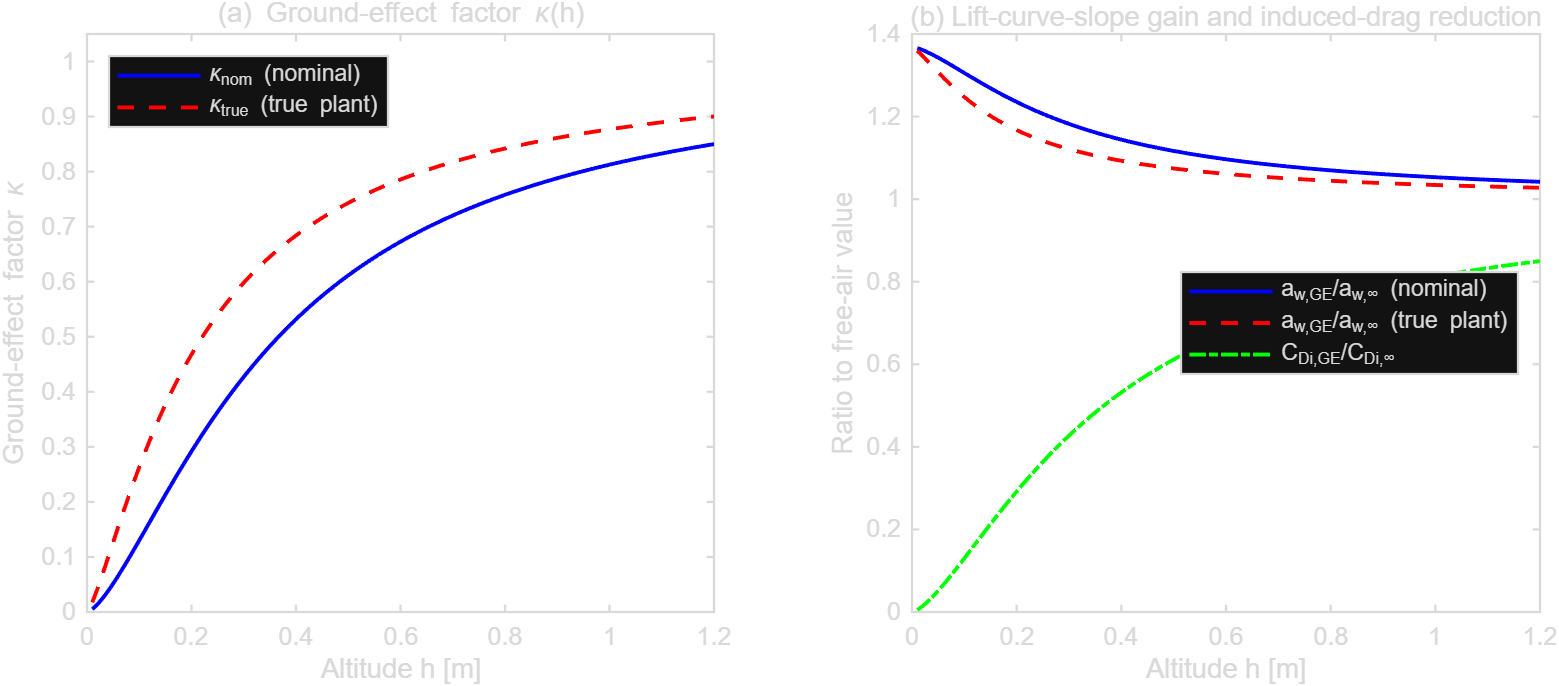
\includegraphics[width=1.00\linewidth]{fig1_ge}
\vspace{2pt}
\caption{Ground-effect factor and the resulting lift-curve-slope gain and induced drag versus height above ground.}
\label{fig:ge}
\end{figure}

\begin{table}[!t]
\centering
\caption{Ground-effect factor and effective lift-curve slope (nominal model and true plant)}
\label{tab:getab}
\footnotesize
\setlength{\tabcolsep}{4pt}
\begin{adjustbox}{max width=\columnwidth}
\wigmeasure{getab}{%
\begin{tabular}{ccccccc}
\toprule
$h$ / m & $h/b$ & $\kappa_{nom}$ & $\kappa_{true}$ & $a_{w,nom}$ & $a_{w,true}$ & $a_w$ gain / \% \\
\midrule
0.05 & 0.0208 & 0.0515 & 0.1266 & 5.7902 & 5.6372 & 34.28 \\
0.10 & 0.0417 & 0.1301 & 0.2630 & 5.6302 & 5.3790 & 30.57 \\
0.15 & 0.0625 & 0.2130 & 0.3768 & 5.4708 & 5.1812 & 26.87 \\
0.20 & 0.0833 & 0.2919 & 0.4677 & 5.3273 & 5.0331 & 23.54 \\
0.50 & 0.2083 & 0.6115 & 0.7431 & 4.8156 & 4.6325 & 11.68 \\
1.20 & 0.5000 & 0.8499 & 0.9002 & 4.4936 & 4.4311 & 4.21 \\
\bottomrule
\end{tabular}}
\end{adjustbox}
\end{table}

\subsection{Seventh-Order Nonlinear Longitudinal Model}
The state vector is $x = [V,\ \gamma,\ \alpha,\ q,\ h,\ T,\ \delta_e]^{T}$ and the control vector is $u = [\delta_{e,c},\ \delta_t]^{T}$. The longitudinal equations of motion are

\begin{equation}
\adjustbox{max width=\columnwidth}{$\displaystyle m\dot{V} = T\cos(\alpha + i_T) - D - mg\sin\gamma$}
\end{equation}

\begin{equation}
\adjustbox{max width=\columnwidth}{$\displaystyle mV\dot{\gamma} = L + T\sin(\alpha + i_T) - mg\cos\gamma$}
\end{equation}

\begin{equation}
\adjustbox{max width=\columnwidth}{$\displaystyle \dot{\alpha} = q - \dot{\gamma}, \qquad I_{yy}\,\dot{q} = M, \qquad \dot{h} = V\sin\gamma$}
\end{equation}

\begin{equation}
\adjustbox{max width=\columnwidth}{$\displaystyle \tau_T \dot{T} = T_{cmd} - T, \qquad \tau_e \dot{\delta}_e = \sat(\delta_{e,c}) - \delta_e$}
\end{equation}

The pitch angle follows from $\theta = \gamma + \alpha$. The wing lift coefficient is $C_{L,w} = a_w(h)(\alpha - \alpha_{L0})$ and the wing drag is $C_{D,w} = C_{D0} + C_{Di}$. The local angle of attack of the tail is

\begin{equation}
\adjustbox{max width=\columnwidth}{$\displaystyle \alpha_t = \alpha + i_t - \varepsilon(h,\alpha) + \frac{q\, l_t}{V}$}
\end{equation}

and its lift coefficient is $C_{L,t} = a_t(h_t)(\alpha_t - \alpha_{L0,t}) + a_{\delta_e}\delta_e$, where the effective tail lift-curve slope is computed from (2) using the tail height $h_t = h + \Delta z_t$ and the tail span. All moments are evaluated as $M = z F_x - x F_z$ and include the wing, the tail, the thrust-line offset and the fuselage. A fixed-step fourth-order Runge-Kutta integrator with a 1 ms step is used, and the flight-control computer runs at 200 Hz with a zero-order hold.

\subsection{Uncertainty Between the Nominal Model and the True Plant}
The controller uses a nominal model while the plant is the true vehicle; the difference is the uncertainty the adaptation law must compensate online. Four classes of mismatch are introduced, namely ground-effect strength mismatch, the RAM effect (extra lift and nose-down moment from the high-pressure region beneath the wing), lift nonlinearity and aerodynamic parameter perturbation; see Table IV.

\begin{table*}[!t]
\centering
\caption{Mismatch between the nominal model and the true plant}
\label{tab:mismatch}
\footnotesize
\setlength{\tabcolsep}{4pt}
\begin{adjustbox}{max width=\textwidth}
\wigmeasure{mismatch}{%
\begin{tabular}{lccl}
\toprule
Mismatch & Nominal & True & Physical meaning \\
\midrule
Ground-effect shape $A$ & 0.0641 & 0.045 & ground-effect strength underestimated \\
Ground-effect exponent $n$ & 1.4622 & 1.300 & different height decay law \\
RAM extra lift & none & $k_{ram} = 0.09$ & extra lift from high-pressure region \\
RAM extra moment & none & acting point shifted 5 cm aft & centre of pressure moves aft \\
Lift nonlinearity & linear & $C_{L,\max} = 1.3$ softening & stall softening at high $\alpha$ \\
Parasite drag $C_{D0}$ & 0.0250 & 0.0320 & drag coefficient +28\% \\
Downwash gradient $\varepsilon_\alpha$ & 0.350 & 0.450 & tail downwash +29\% \\
\bottomrule
\end{tabular}}
\end{adjustbox}
\end{table*}

At the trim points the mismatch of the true plant relative to the nominal model is: pitch-moment mismatch $|\Delta M| \le 0.8742$ N$\cdot$m, peak lift mismatch $|\Delta L| \approx 13.89$ N (11.8\% of weight), and drag mismatch about 1.57 to 2.03 N. This level of mismatch represents a typical situation in which an engineering estimate has not been calibrated against CFD.

\section{Mechanism of Ground-Effect Height Instability}
\subsection{Trim Characteristics}
For steady level flight ($\gamma = 0$, $q = 0$) the trim conditions are

\begin{equation}
\adjustbox{max width=\columnwidth}{$\displaystyle T\cos(\alpha + i_T) - D = 0, \quad L + T\sin(\alpha + i_T) - mg = 0, \quad M = 0$}
\end{equation}

which are solved for $\alpha$, $\delta_e$ and $T$. Table V lists the trim results and the ground-effect height derivative at $V = 18$ m/s.

\begin{table*}[!t]
\centering
\caption{Trim results and ground-effect height derivative versus height ($\partial M/\partial h$ in N$\cdot$m/m)}
\label{tab:trimtab}
\footnotesize
\setlength{\tabcolsep}{4pt}
\begin{adjustbox}{max width=\textwidth}
\wigmeasure{trimtab}{%
\begin{tabular}{cccccccc}
\toprule
$h$ / m & $\alpha_{nom}$ / deg & $\alpha_{true}$ / deg & $\delta_{e,nom}$ / deg & $\delta_{e,true}$ / deg & $(L/D)_{nom}$ & $(L/D)_{true}$ & $\partial M/\partial h$ \\
\midrule
0.05 & 3.160 & 3.109 & -3.778 & -4.701 & 21.97 & 16.59 & +14.901 \\
0.15 & 3.516 & 3.846 & -3.674 & -4.445 & 19.27 & 14.22 & +12.795 \\
0.25 & 3.847 & 4.427 & -3.506 & -4.169 & 17.29 & 12.81 & +8.994 \\
0.35 & 4.110 & 4.822 & -3.320 & -3.915 & 15.99 & 11.96 & +6.188 \\
0.45 & 4.310 & 5.086 & -3.146 & -3.700 & 15.12 & 11.43 & +4.358 \\
0.55 & 4.462 & 5.267 & -2.995 & -3.525 & 14.52 & 11.08 & +3.170 \\
\bottomrule
\end{tabular}}
\end{adjustbox}
\end{table*}

As height increases the ground effect weakens: the trim angle of attack rises from 3.160 to 4.462 deg and the lift-to-drag ratio falls from 21.97 to 14.52. Because of the ground-effect mismatch and the RAM effect, the trim elevator of the true plant differs from the nominal value by 0.53 to 0.92 deg, which is exactly the steady-state mismatch the controller has to compensate.

\begin{figure}[!t]
\centering
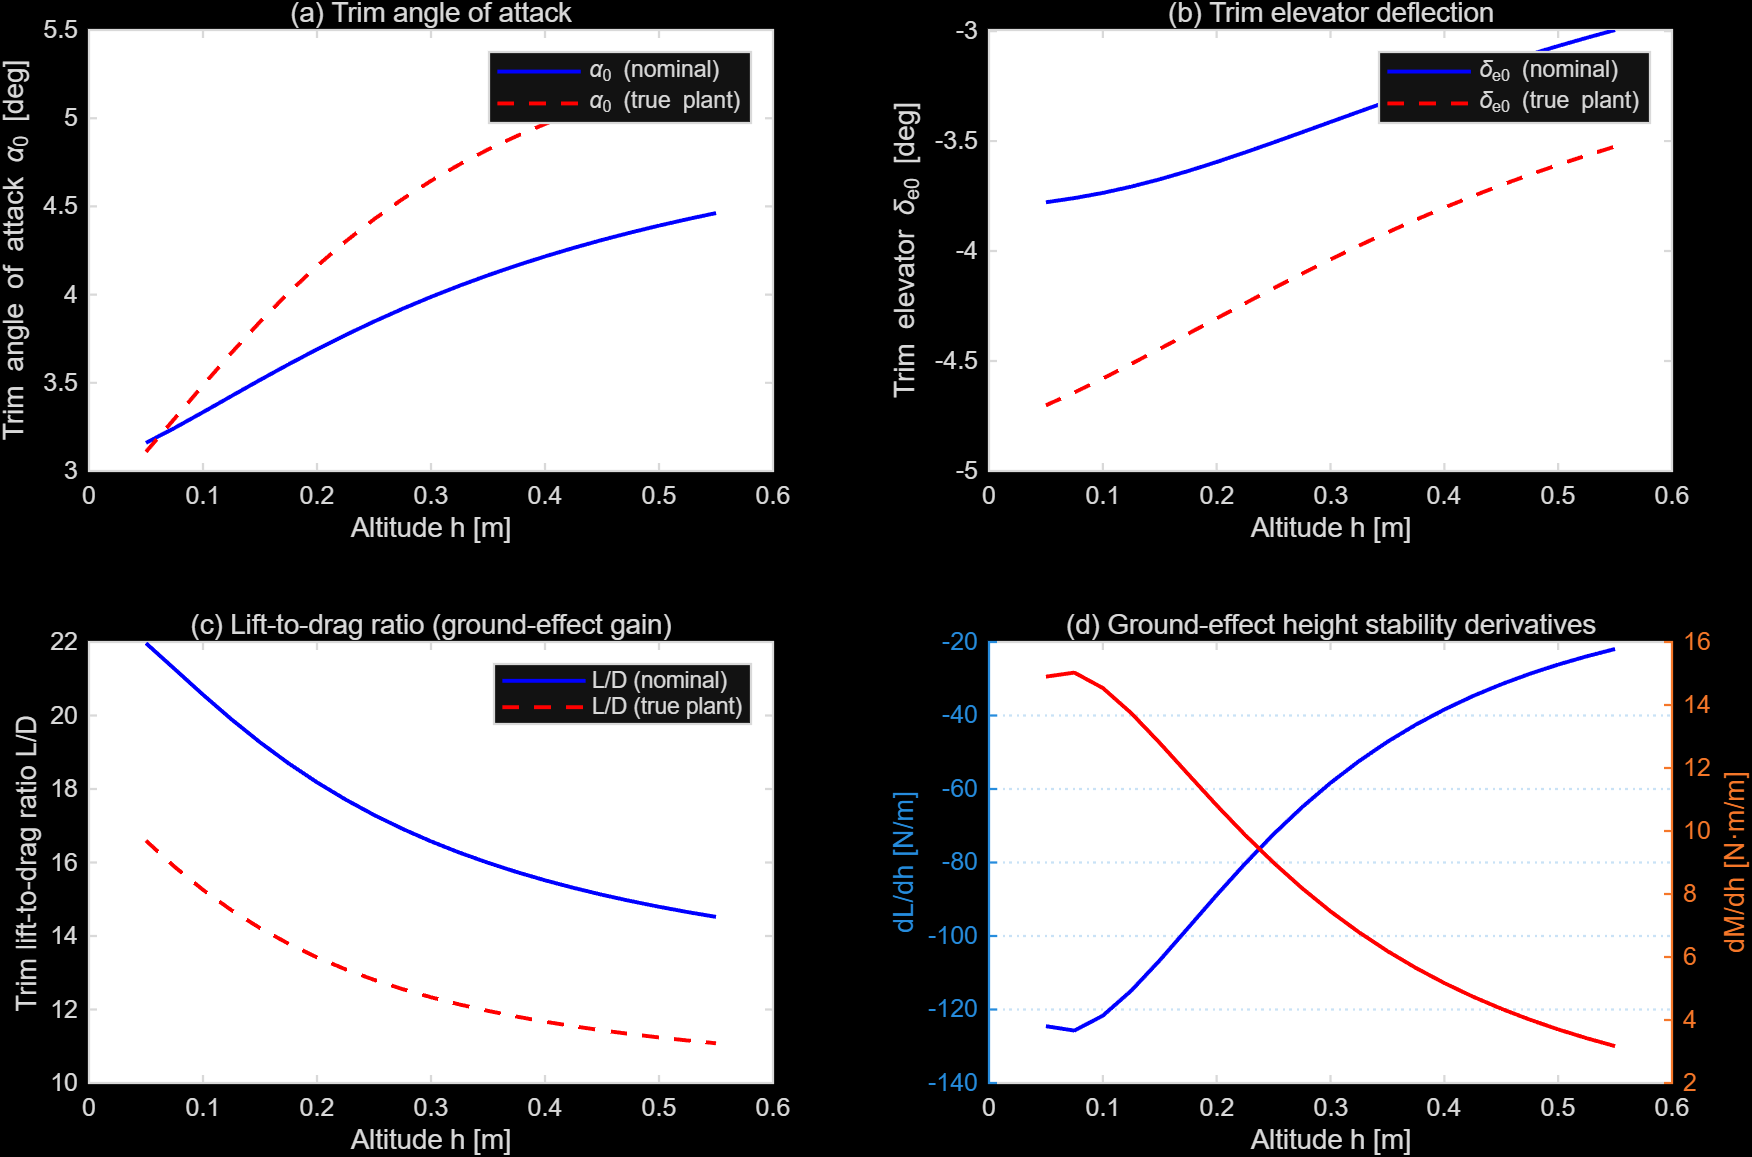
\includegraphics[width=1.00\linewidth]{fig2_trim}
\vspace{2pt}
\caption{Trim characteristics and ground-effect height derivative versus height above ground.}
\label{fig:trim}
\end{figure}

\subsection{Component-Wise Decomposition of $\partial M/\partial h$}
The last column of Table V shows that over the whole envelope $\partial M/\partial h = +3.17$ to +14.90 N$\cdot$m/m, always positive: a reduction in height produces an additional nose-down moment, closing a positive height-pitch feedback loop, i.e. the classical ground-effect height instability. To locate its physical origin the pitch moment is differentiated component by component at the trim point (central differences in $h$, all other states frozen):

\begin{equation}
\adjustbox{max width=\columnwidth}{$\displaystyle \frac{\partial M}{\partial h} = \frac{\partial M_w}{\partial h} + \frac{\partial M_t}{\partial h} + \frac{\partial M_{ram}}{\partial h} + \frac{\partial M_{nl}}{\partial h}$}
\end{equation}

where the subscripts $w$, $t$, $ram$ and $nl$ denote the wing, the tail, the RAM force and the lift-softening residual respectively. The fuselage and thrust-line terms are independent of $h$ and vanish identically. Table VI gives the decomposition.

\begin{table}[!t]
\centering
\caption{Component-wise decomposition of the pitch-moment height derivative (all values in N$\cdot$m/m)}
\label{tab:decomp}
\footnotesize
\setlength{\tabcolsep}{4pt}
\begin{adjustbox}{max width=\columnwidth}
\wigmeasure{decomp}{%
\begin{tabular}{ccccccc}
\toprule
$h$ / m & $\partial M/\partial h$ & Wing & Tail & RAM & Nonlinear & Tail share / \% \\
\midrule
0.05 & +14.90 & -2.30 & +15.78 & +0.76 & +0.66 & 105.9 \\
0.15 & +12.79 & -1.54 & +12.43 & +1.33 & +0.57 & 97.2 \\
0.25 & +8.99 & -0.95 & +8.54 & +1.03 & +0.38 & 95.0 \\
0.35 & +6.19 & -0.62 & +5.91 & +0.66 & +0.25 & 95.5 \\
0.45 & +4.36 & -0.42 & +4.21 & +0.41 & +0.16 & 96.6 \\
0.55 & +3.17 & -0.30 & +3.10 & +0.26 & +0.11 & 97.8 \\
0.80 & +1.63 & -0.15 & +1.62 & +0.10 & +0.05 & 99.9 \\
1.00 & +1.06 & -0.10 & +1.07 & +0.06 & +0.03 & 101.0 \\
\bottomrule
\end{tabular}}
\end{adjustbox}
\end{table}

The decomposition is unambiguous. The tail term is the largest positive contribution at every height (+1.07 to +15.78 N$\cdot$m/m, i.e. 95.0\% to 105.9\% of the total), whereas the wing term is always negative (-2.30 to -0.10 N$\cdot$m/m) and therefore stabilising. The physical mechanisms are as follows.

\begin{itemize}
  \item \textbf{Tail (destabilising).} Flying close to the ground reduces the downwash at the tail, which increases the local tail incidence. In trim the tail carries a negative lift (downwash load), so an increased incidence weakens that negative lift and produces an additional nose-down moment.
  \item \textbf{Wing (stabilising).} Ground effect increases lift ($\partial L_w/\partial h < 0$) while the wing aerodynamic centre lies 2 cm ahead of the centre of gravity, so the extra lift produces a nose-up moment.
  \item \textbf{RAM (destabilising).} The high-pressure region beneath the wing acts aft of the aerodynamic centre and strengthens as height decreases, producing a nose-down moment.
  \item \textbf{Lift nonlinearity (destabilising).} Stall softening is stronger at low height, which is equivalent to losing part of the lift; its point of action is ahead of the aerodynamic centre, so it also produces a nose-down moment.
\end{itemize}

The sum of the four components matches the total derivative to within 2.4e-12 N$\cdot$m/m, which verifies the consistency of the decomposition. The practical implication is that height stability should be improved primarily through the tail layout (for example a larger tail height offset, downwash shielding, or an all-moving tail) rather than by reshaping the wing planform.

\begin{figure}[!t]
\centering
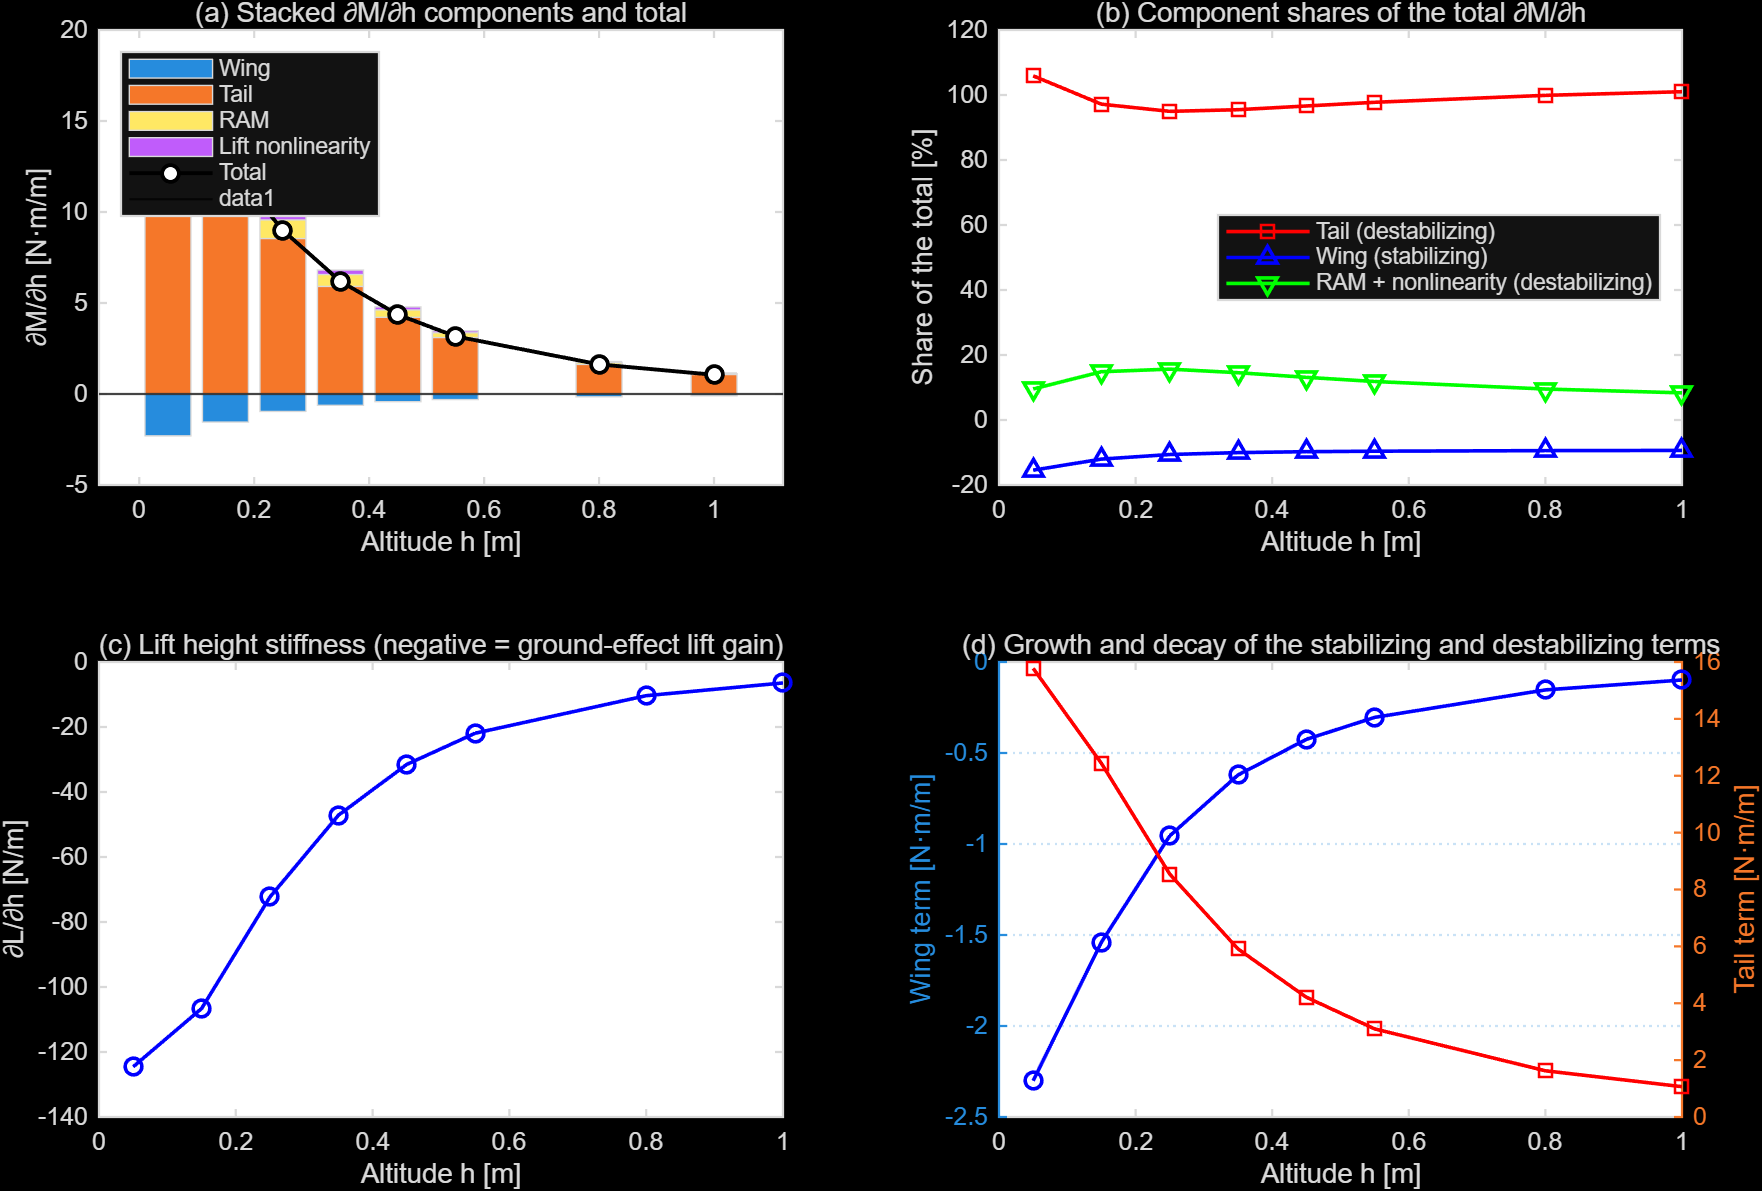
\includegraphics[width=1.00\linewidth]{fig12_mdh}
\vspace{2pt}
\caption{Stacked components and shares of $\partial M/\partial h$, and the lift height stiffness.}
\label{fig:mdh}
\end{figure}

\subsection{Instability of the Phugoid-Height Coupled Mode}
Numerical linearisation of (3)-(7) at the trim points gives the longitudinal modes. To isolate the role of the ground effect, the modes are also computed with the ground effect effectively switched off ($A \to 0$, i.e. $\kappa \equiv 1$).

\begin{table}[!t]
\centering
\caption{Low-frequency (phugoid-height coupled) mode versus height}
\label{tab:modes}
\footnotesize
\setlength{\tabcolsep}{4pt}
\begin{adjustbox}{max width=\columnwidth}
\wigmeasure{modes}{%
\begin{tabular}{cccccc}
\toprule
$h$ / m & With GE, real / (1/s) & imag / (1/s) & damping & No GE, real / (1/s) & imag / (1/s) \\
\midrule
0.05 & +0.4463 & 0.5774 & -0.612 & -0.0027 & 0.9303 \\
0.10 & +0.4704 & 0.4970 & -0.687 & -0.0094 & 1.0564 \\
0.15 & +0.4818 & 0.4228 & -0.752 & -0.0113 & 1.0850 \\
0.20 & +0.4875 & 0.3507 & -0.812 & -0.0077 & 1.0583 \\
0.25 & +0.4861 & 0.2845 & -0.863 & -0.0032 & 1.0080 \\
0.30 & +0.4767 & 0.2308 & -0.900 & -0.0004 & 0.9529 \\
0.35 & +0.4607 & 0.1947 & -0.921 & +0.0002 & 0.9020 \\
0.40 & +0.4399 & 0.1780 & -0.927 & -0.0011 & 0.8584 \\
0.45 & +0.4160 & 0.1778 & -0.919 & -0.0036 & 0.8226 \\
0.50 & +0.3905 & 0.1882 & -0.901 & -0.0066 & 0.7937 \\
0.55 & +0.3643 & 0.2037 & -0.873 & -0.0098 & 0.7706 \\
0.60 & +0.3379 & 0.2208 & -0.837 & -0.0128 & 0.7523 \\
0.65 & +0.3118 & 0.2379 & -0.795 & -0.0156 & 0.7377 \\
0.70 & +0.2861 & 0.2541 & -0.748 & -0.0181 & 0.7260 \\
0.75 & +0.2609 & 0.2694 & -0.696 & -0.0203 & 0.7166 \\
0.80 & +0.2363 & 0.2837 & -0.640 & -0.0222 & 0.7091 \\
0.85 & +0.2123 & 0.2972 & -0.581 & -0.0239 & 0.7029 \\
0.90 & +0.1888 & 0.3101 & -0.520 & -0.0253 & 0.6978 \\
0.95 & +0.1658 & 0.3227 & -0.457 & -0.0265 & 0.6936 \\
1.00 & +0.1434 & 0.3354 & -0.393 & -0.0275 & 0.6901 \\
\bottomrule
\end{tabular}}
\end{adjustbox}
\end{table}

The conclusion is clear:

\begin{itemize}
  \item With the ground effect switched off, the real part of the low-frequency mode is -0.0275 to +0.0002 1/s, i.e. neutral stability, of the same order as the classical phugoid estimate ($\omega_p = \sqrt{2}g/V = 0.7705$ rad/s and the Lanchester approximation $\zeta_p = 1/(\sqrt{2}(L/D)) = 0.0404$ to $0.0690$).
  \item With the ground effect active the real part becomes +0.1434 to +0.4875 1/s and the damping ratio drops to -0.927, so the instability is caused entirely by the ground effect.
  \item The largest real part occurs at $h \approx 0.20$ m (+0.4875 1/s, a time constant of about 2.05 s) with an oscillation frequency of 0.178 to 0.577 rad/s, which is a typical phugoid-height coupled oscillation.
\end{itemize}

\begin{figure}[!t]
\centering
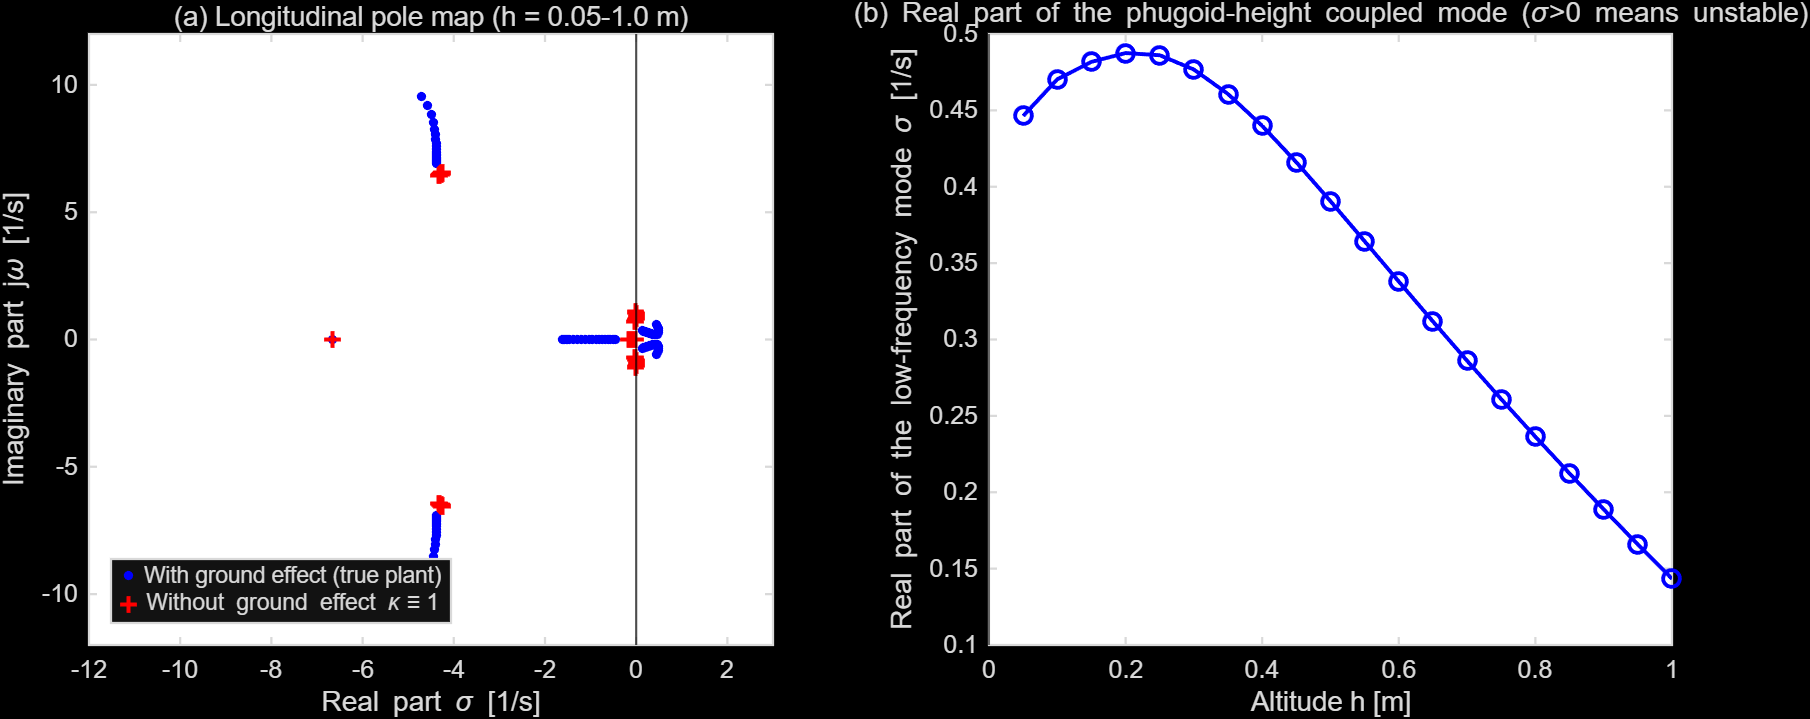
\includegraphics[width=1.00\linewidth]{fig3_modes}
\vspace{2pt}
\caption{Longitudinal pole map and the real part of the phugoid-height coupled mode versus height.}
\label{fig:modes}
\end{figure}

This result is consistent with the moment decomposition of Section III-B: the height variation of the tail downwash both supplies most of $\partial M/\partial h > 0$ and pushes the otherwise neutrally stable phugoid mode into the right half-plane through the height-normal-force coupling. A WIG vehicle must therefore rely on active height control whose bandwidth covers this mode frequency with adequate phase margin.

\section{RBF Neural-Network Adaptive Controller Design}
\subsection{Control Architecture}
The controller has a three-layer cascade structure:

\begin{itemize}
  \item \textbf{Altitude outer loop} (kinematic): the height error and height rate generate the flight-path angle command $\gamma_c$;
  \item \textbf{attitude inner loop} (dynamic surface + dynamic inversion + RBF + robust term): $\gamma_c$ generates the pitch-angle command $\theta_c$, and the pitch-rate loop then solves for the elevator command $\delta_{e,c}$;
  \item \textbf{airspeed loop} (thrust dynamic inversion + RBF + robust term + integral): the speed error generates the throttle command $\delta_t$.
\end{itemize}

Two RBF networks are used [7], [8], [14]: a moment channel with inputs $[\alpha, q, h]$ and $5 \times 3 \times 5 = 75$ nodes, estimating the pitch-moment mismatch, and a drag channel with inputs $[\alpha, V, h]$ and $4 \times 4 \times 4 = 64$ nodes, estimating the drag mismatch. \textbf{No separate lift channel is required}, because the angle-of-attack feedback in $\theta_d = \gamma_c + \alpha$ of (11) compensates it automatically. The reason deserves emphasis: if the pitch loop tracks $\theta = \theta_d$, then the kinematic identity $\gamma = \theta - \alpha$ immediately gives $\gamma = \gamma_c$. Since this derivation uses only $\gamma = \theta - \alpha$ and is independent of both the control law and the model, the flight-path angle still tracks its command accurately even when the lift model is in error (the angle of attack simply changes), which removes an entire network.

\subsection{Altitude Outer Loop and Dynamic-Surface Attitude Inner Loop}
The altitude loop is a proportional guidance law with height-rate damping; the height rate is synthesised directly from $\dot{h} = V\sin\gamma$ so that no numerical differentiation is needed:

\begin{equation}
\adjustbox{max width=\columnwidth}{$\displaystyle \gamma_d = \arcsin\!\left[\sat\!\left(\frac{\dot{h}_c - k_h e_h - k_{hd}(\dot{h} - \dot{h}_c)}{V},\ \sin\gamma_{\max}\right)\right], \qquad e_h = h - h_c$}
\end{equation}

The attitude loop uses dynamic surface control (DSC) [11]-[13] so that the virtual control need not be differentiated analytically:

\begin{equation}
\adjustbox{max width=\columnwidth}{$\displaystyle \theta_d = \sat\!\left(\gamma_c + \alpha,\ \theta_{\max}\right), \qquad \tau_{th}\dot{\theta}_c = \theta_d - \theta_c$}
\end{equation}

\begin{equation}
\adjustbox{max width=\columnwidth}{$\displaystyle q_d = \dot{\theta}_c - k_\theta(\theta - \theta_c), \qquad \tau_q \dot{q}_{cf} = \sat(q_d) - q_{cf}$}
\end{equation}

\begin{equation}
\adjustbox{max width=\columnwidth}{$\displaystyle e_q = q - q_{cf}, \qquad \nu = \dot{q}_{cf} - k_q e_q$}
\end{equation}

Since $\gamma = \theta - \alpha$, (11) implies $\dot{\theta} = k_\theta(\gamma_c - \gamma)$: the pitch loop is equivalent to a flight-path-angle tracking loop with natural frequency and damping $\omega_n = \sqrt{\dot{\gamma}_\alpha k_\theta}$ and $\zeta = \dot{\gamma}_\alpha/(2\omega_n)$, where $\dot{\gamma}_\alpha = \partial\dot{\gamma}/\partial\alpha = 3.9051$ 1/s is obtained from the numerical linearisation. With $k_\theta = 3.20$ 1/s this gives $\omega_n = 3.535$ rad/s and $\zeta = 0.552$; tuning requires $\zeta \geq 1$ so that this loop does not resonate (Section IV-E).

\subsection{Dynamic-Inversion Control Law and Adaptation Law}
Let $M_0(x)$ be the nominal zero-elevator pitch moment and $M_{\delta_e}$ the control derivative, and define $f_0 = M_0/I_{yy}$ and $b = M_{\delta_e}/I_{yy}$. The elevator command is

\begin{equation}
\adjustbox{max width=\columnwidth}{$\displaystyle \delta_{e,c} = \frac{1}{b}\left(\nu - f_0 - u_M - u_r\right)$}
\end{equation}

where $u_M = W_1^{T}\phi_1$ is the online estimate of the moment mismatch and $u_r$ is the robust term. The basis functions and the regression vector are

\begin{equation}
\adjustbox{max width=\columnwidth}{$\displaystyle \phi_j(z) = \exp\!\left(-\frac{1}{2}\sum_{i=1}^{3}\frac{(z_i - c_{ij})^{2}}{\sigma_i^{2}}\right), \qquad \phi_1 = \phi(z_1)\,\frac{\bar{q}Sc}{I_{yy}}$}
\end{equation}

The centres $c_j$ are placed on a uniform grid in the normalised cube $[-1,1]^3$ and the widths are set to the grid spacing, so that neighbouring basis functions overlap by $e^{-1/2} \approx 0.61$ at their centres. Including $\bar{q}Sc$ in the regression vector is a physical dimensionality reduction: since the aerodynamic moment is proportional to dynamic pressure, factoring it out leaves the network to learn only the non-dimensional moment-coefficient mismatch, which keeps the weight magnitudes stable across speed and reduces the moment-channel input dimension from four to three, cutting the node count by an order of magnitude. The weights are kept bounded by a projection operator [9], [10]:

\begin{equation}
\adjustbox{max width=\columnwidth}{$\displaystyle \dot{W}_1 = \Proj\!\left[\Gamma_1\left(\phi_1 e_q - \nu_e|e_q| W_1\right)\right],\qquad \dot{W}_2 = -\Gamma_2\left(\phi_2 e_V + \nu_e|e_V| W_2\right)$}
\end{equation}

\begin{equation}
\adjustbox{max width=\columnwidth}{$\displaystyle \Proj(\tau) = \begin{cases} \tau, & \left\|W\right\| < W_{\max}\ \text{or}\ W^{T}\tau \leq 0 \\ \tau - \dfrac{W W^{T}}{\left\|W\right\|^{2}}\tau, & \text{otherwise} \end{cases}$}
\end{equation}

Note that the signs of the two adaptation laws are opposite, because the estimates enter the control laws in different positions: $u_M$ enters (14) with a minus sign while $u_D$ enters (18) with a plus sign. If a sign is wrong the estimate becomes positive feedback and the closed loop diverges.

\subsection{Airspeed Loop}
The airspeed control law and error dynamics are

\begin{equation}
\adjustbox{max width=\columnwidth}{$\displaystyle T_{cmd} = \frac{m\left(\dot{V}_d + u_D - u_{rV}\right) + D_0 + mg\sin\gamma_c}{\cos(\alpha + i_T)}$}
\end{equation}

\begin{equation}
\adjustbox{max width=\columnwidth}{$\displaystyle \dot{V}_d = \dot{V}_c - k_V e_V - k_{IV} I_V, \qquad \dot{I}_V = e_V$}
\end{equation}

Two details of (18) are essential. First, the gravity feedforward must be taken from the commanded flight-path angle $\gamma_c$, not from the measured $\gamma$: using the measurement closes a positive feedback loop $\gamma \to T_{cmd} \to T \to V \to L \to \dot{\gamma} \to \gamma$ with a loop gain of $mg = 117.7$ N/rad, which, together with the engine lag, pushes the short-period/phugoid coupled mode into the right half-plane. Second, the robust term must enter with a minus sign so that $-u_{rV}$ appears in the error dynamics, matching the moment channel and making the Lyapunov cross-terms cancel exactly.

\subsection{Lyapunov Stability Analysis}
Let the moment mismatch between the true plant and the nominal model be $\Delta f = \Delta M/I_{yy}$ and the drag mismatch be $\Delta D/m$, and write the ideal approximation as $\Delta f = W_1^{*T}\phi_1 + \varepsilon_1$ and $\Delta D/m = W_2^{*T}\phi_2 + \varepsilon_2$, with weight error $\tilde{W}_i = W_i - W_i^{*}$. Substituting into (14) and (18) gives the error dynamics

\begin{equation}
\adjustbox{max width=\columnwidth}{$\displaystyle \dot{e}_q = -k_q e_q - \tilde{W}_1^{T}\phi_1 + \varepsilon_1 - u_r$}
\end{equation}

\begin{equation}
\adjustbox{max width=\columnwidth}{$\displaystyle \dot{e}_V = -k_V e_V - k_{IV} I_V + \tilde{W}_2^{T}\phi_2 - \varepsilon_2 - u_{rV}$}
\end{equation}

Consider the Lyapunov function

\begin{equation}
\adjustbox{max width=\columnwidth}{$\displaystyle V_L = \frac{1}{2}e_q^{2} + \frac{1}{2}\tilde{W}_1^{T}\Gamma_1^{-1}\tilde{W}_1 + \frac{1}{2}e_V^{2} + \frac{1}{2}\tilde{W}_2^{T}\Gamma_2^{-1}\tilde{W}_2 + \frac{1}{2}k_{IV} I_V^{2}$}
\end{equation}

Differentiating along the closed-loop trajectories and substituting (16), the cross-terms cancel exactly:

\begin{equation}
\adjustbox{max width=\columnwidth}{$\displaystyle e_q\left(-\tilde{W}_1^{T}\phi_1\right) + \tilde{W}_1^{T}\Gamma_1^{-1}\Gamma_1\phi_1 e_q = 0$}
\end{equation}

\begin{equation}
\adjustbox{max width=\columnwidth}{$\displaystyle e_V\left(\tilde{W}_2^{T}\phi_2\right) + \tilde{W}_2^{T}\Gamma_2^{-1}\left(-\Gamma_2\phi_2 e_V\right) = 0$}
\end{equation}

Equations (23) and (24) are exactly why the signs of the two adaptation laws must be opposite. The $e$-modification gives $\tilde{W}_i^{T}W_i \geq \frac{1}{2}\|\tilde{W}_i\|^2 - \frac{1}{2}\|W_i^{*}\|^2$. In addition the standard inequality $|z| - z\tanh(z/\Phi) \leq 0.2785\,\Phi$ is used, for which a self-contained proof is as follows: with $u = z/\Phi \geq 0$ the left-hand side equals $\Phi\,g(u)$ where $g(u) = u(1 - \tanh u)$; setting $g'(u) = 1 - \tanh u - u\,\mathrm{sech}^{2}u = 0$ gives $u^{*} = 1/(1 + \tanh u^{*}) \approx 0.6392$ and $g(u^{*}) \approx 0.278465$, so $0.2785$ is the exact bound. Provided the robust gains satisfy $\eta_r \geq \varepsilon_N + d_M$ and $\eta_V \geq \varepsilon_N + d_V$, one obtains

\begin{equation}
\adjustbox{max width=\columnwidth}{$\displaystyle \dot{V}_L \leq -2\lambda_{\min} V_L + c_0, \qquad c_0 = 0.2785\left(\eta_r\Phi_r + \eta_V\Phi_V\right) + \nu_e\left(\left\|W_1^{*}\right\|^{2} + \left\|W_2^{*}\right\|^{2}\right)$}
\end{equation}

where $\lambda_{\min} = \min\{k_q, k_V, k_{IV}, \nu_e\}/2$ is a lower bound on the decay rate. Hence the uniform ultimate boundedness (UUB) result

\begin{equation}
\adjustbox{max width=\columnwidth}{$\displaystyle \left\|e(t)\right\| \leq \sqrt{\frac{2V_L(0)}{\lambda_{\min}}e^{-2\lambda_{\min} t} + \frac{c_0}{\lambda_{\min}}}$}
\end{equation}

that is, the tracking error converges exponentially to a residual set of radius $\sqrt{c_0/\lambda_{\min}}$. The projection operator (17) guarantees $\|W(t)\| \leq W_{\max}$ for all $t \geq 0$, and its geometric property of removing only the radial component does not destroy the negative definiteness of $\dot{V}_L$. The altitude loop is a cascade: from $\dot{e}_h = -k_h e_h + V(\sin\gamma - \sin\gamma_c)$ the height error is ultimately bounded by the inner-loop flight-path tracking error, so the UUB property of the inner loop carries over to the whole closed loop.

The $\nu_e$ term in (25) makes $c_0$ depend on the ideal weight norms, which gives a design hint: the $e$-modification coefficient should not be too large, otherwise the residual radius is dominated by $\nu_e\|W^{*}\|^2/\lambda_{\min}$. Here $\nu_e = 0.50$ and the measured weight norms settle at $\|W_1\| \approx 0.044$ and $\|W_2\| \approx 0.150$, far below the projection bound $W_{\max} = 12.0$, so the residual radius is governed mainly by the robust-term contribution $0.2785(\eta_r\Phi_r + \eta_V\Phi_V)$.

\subsection{Discrete-Time Stability Constraint}
The adaptation law is implemented digitally at 200 Hz with forward Euler. This is the step most easily overlooked when moving an RBF adaptive design from continuous time to a digital implementation, and it has the most severe consequences [15]-[17]. Combining the error and weight channels and linearising (all other dynamics frozen, leakage and projection neglected) gives the two-state system

\begin{equation}
\adjustbox{max width=\columnwidth}{$\displaystyle \begin{bmatrix} e(k+1) \\ \tilde{W}(k+1) \end{bmatrix} = \begin{bmatrix} 1 - T_s k & -T_s\phi^{T} \\ T_s\Gamma\phi & 1 \end{bmatrix}\begin{bmatrix} e(k) \\ \tilde{W}(k) \end{bmatrix}$}
\end{equation}

whose characteristic polynomial is $\lambda^2 - (1-T_sk)\lambda + (1 - T_sk + T_s^2\Gamma\|\phi\|^2)$. The Jury criterion, through $\det < 1$, yields the governing constraint

\begin{equation}
\adjustbox{max width=\columnwidth}{$\displaystyle T_s\,\Gamma_i\left\|\phi_i\right\|^{2} < k_i$}
\end{equation}

where $k_1 = k_q$ and $k_2 = k_V$ are the proportional gains of the corresponding channels. Writing each regression vector as a dimensional factor times the basis vector, $\phi_1 = \phi_{rbf}\,\bar{q}Sc/I_{yy}$ and $\phi_2 = \phi_{rbf}/m$, and substituting the parameters used here:

\begin{table}[!t]
\centering
\caption{Stability margins of the discrete adaptation law at the trim point ($T_s = 5$ ms)}
\label{tab:disc}
\footnotesize
\setlength{\tabcolsep}{4pt}
\begin{adjustbox}{max width=\columnwidth}
\wigmeasure{disc}{%
\begin{tabular}{cccccc}
\toprule
Channel & Factor $g_i$ & $\|\phi_{i,rbf}\|^2$ & $T_s\Gamma_i\|\phi_i\|^2$ & Gain $k_i$ & Margin ratio \\
\midrule
Moment & 66.265 s$^{-2}$ & 5.3943 & 0.5922 & 6.00 & 10.1 \\
Drag & 0.083333 kg$^{-1}$ & 5.3744 & 0.0005598 & 1.53 & 2733.1 \\
\bottomrule
\end{tabular}}
\end{adjustbox}
\end{table}

Table VIII explains quantitatively why the two channel gains differ by three orders of magnitude ($\Gamma_1 = 0.005$ and $\Gamma_2 = 3.0$). The moment-channel regression vector is amplified by $\bar{q}Sc/I_{yy} \approx 66.3$ whereas the drag-channel one is attenuated by $1/m \approx 0.0833$, a ratio of about 795. Comparing the gain values directly would wrongly suggest that the moment channel learns too slowly, and increasing $\Gamma_1$ accordingly drives the weights into saturation within a few sampling periods. Exactly this behaviour was observed during tuning: the weights hit the projection bound and the elevator saturated. Equation (28) provides a directly usable design criterion.

\subsection{Gain Tuning via Sampled Closed-Loop Poles}
For objective assessment of the controller, a sampled-data linearisation of the loop "continuous plant + 200 Hz discrete controller (zero-order hold)" is constructed: a closed-loop simulation with a constant reference is first run until the weights converge, the true equilibrium of the frozen-parameter system is then solved for, and finally the Jacobian of the map $F:(x_k,z_k) \to (x_{k+1},z_{k+1})$ is obtained by central differences and the eigenvalues of the $15 \times 15$ closed-loop matrix are computed. The tuning procedure is:

\begin{enumerate}
  \item Locate the source of instability by switching terms on and off: a pair of unstable poles dominated by the thrust state was found, and the eigenvector confirmed that it was caused by the $mg\sin\gamma$ gravity feedforward in the thrust command closing a positive feedback loop; feeding forward the commanded flight-path angle $\gamma_c$ instead breaks the loop.
  \item Correct the sign of the robust term in the airspeed channel: the robust term must enter the thrust command with a minus sign; written with a plus sign its zero-crossing equivalent gain $\eta_V/\Phi_V$ cancels the airspeed proportional gain and creates positive feedback.
  \item Sweep the nonlinear performance indices over the envelope and select the gains from the height RMS error together with the minimum height above ground.
  \item Set the boundary-layer thicknesses from the rule that the zero-crossing equivalent gain of the robust term must not exceed the proportional gain of that loop: $\Phi_r = 0.80$ rad/s and $\Phi_V = 1.00$ m/s, giving equivalent gains of 3.12 and 1.50.
\end{enumerate}

With the final gains the largest modulus of the 15 sampled closed-loop poles is $\max|z| = 0.99942 < 1$, so all poles lie inside the unit circle; the slowest mode is dominated by the airspeed integral state ($s = -0.116$ 1/s, a time constant of about 8.6 s). The equilibrium residual is 6.6e-17 and the equilibrium height differs from its command by 7.63 mm. A term-by-term sensitivity study further shows that \textbf{switching the robust term off raises $\max|z|$ to 1.00415}, with the dominant pole moving to $s = +0.828$ 1/s and being dominated by the thrust state $T$. The robust term is therefore what keeps this loop stable, which corroborates the conclusion of Section IV-D that the airspeed-channel robust term must enter with a minus sign: if the sign is reversed, its zero-crossing equivalent gain $\eta_V/\Phi_V$ cancels the airspeed proportional gain and the thrust-speed loop loses its damping.

It is worth noting that the closed-loop pole analysis gives different verdicts on the two baselines: the shipped gains give $\max|z| < 1$ (stable), whereas the intermediate tuning gains ($k_h = 3.0$, $\tau_g = 0.05$ s) give $\max|z| = 0.99982$ — still inside the unit circle but only $1.8\times10^{-4}$ from the boundary, i.e. marginal. This motivated reducing $k_h$ from 3.0 to 2.0 and $\tau_g$ from 0.05 s to 0.010 s, which moves the slowest pole from $s = -0.036$ 1/s to $-0.116$ 1/s and markedly improves the margin.

\section{Simulation Validation}
\subsection{Simulation Setup}
Unless stated otherwise the simulations use the "true plant with nominal controller" mismatch configuration: the plant includes ground-effect strength mismatch, the RAM effect and lift nonlinearity, while the controller uses the nominal model. The integration step is 1 ms and the controller samples at 200 Hz. The reference case is a height command of 0.20, 0.35, 0.10 and 0.25 m (spanning the whole ground-effect band) with a speed command of 18 to 20 m/s.

\subsection{Ablation Study}
Table I compares the three control schemes [22], [25], [26]. With the nominal dynamic inversion alone the lift and moment errors caused by the ground-effect mismatch cannot be compensated, and the vehicle loses height in the descent segment and touches the ground. Adding the robust term reduces the error slightly but the vehicle still touches down. With the RBF adaptation the height RMS error falls to 0.0100 m and the minimum height above ground, 0.1000 m, coincides exactly with the lowest commanded height, so no ground contact occurs. The improvement factors are 19.38 in height and 0.39 in airspeed.

\begin{figure}[!t]
\centering
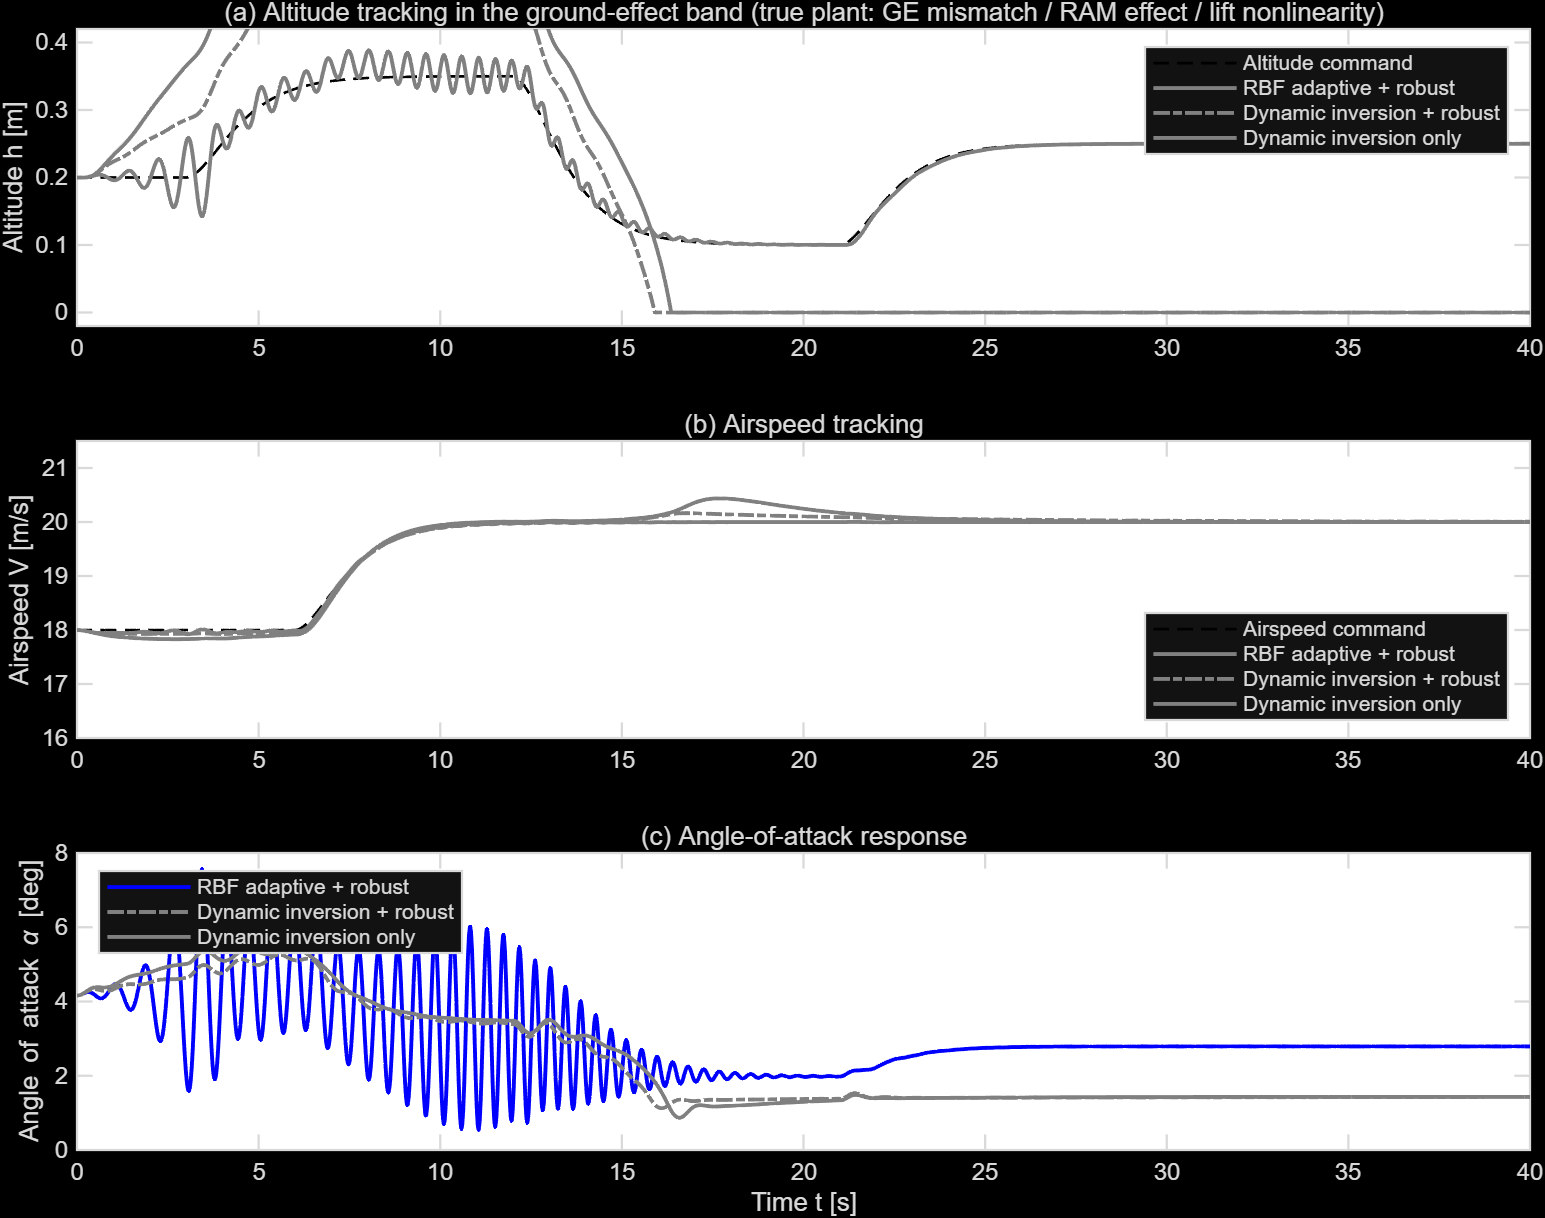
\includegraphics[width=1.00\linewidth]{fig4_tracking}
\vspace{2pt}
\caption{Height and airspeed tracking in the ground-effect band (adaptive versus ablated schemes).}
\label{fig:tracking}
\end{figure}

\begin{figure}[!t]
\centering
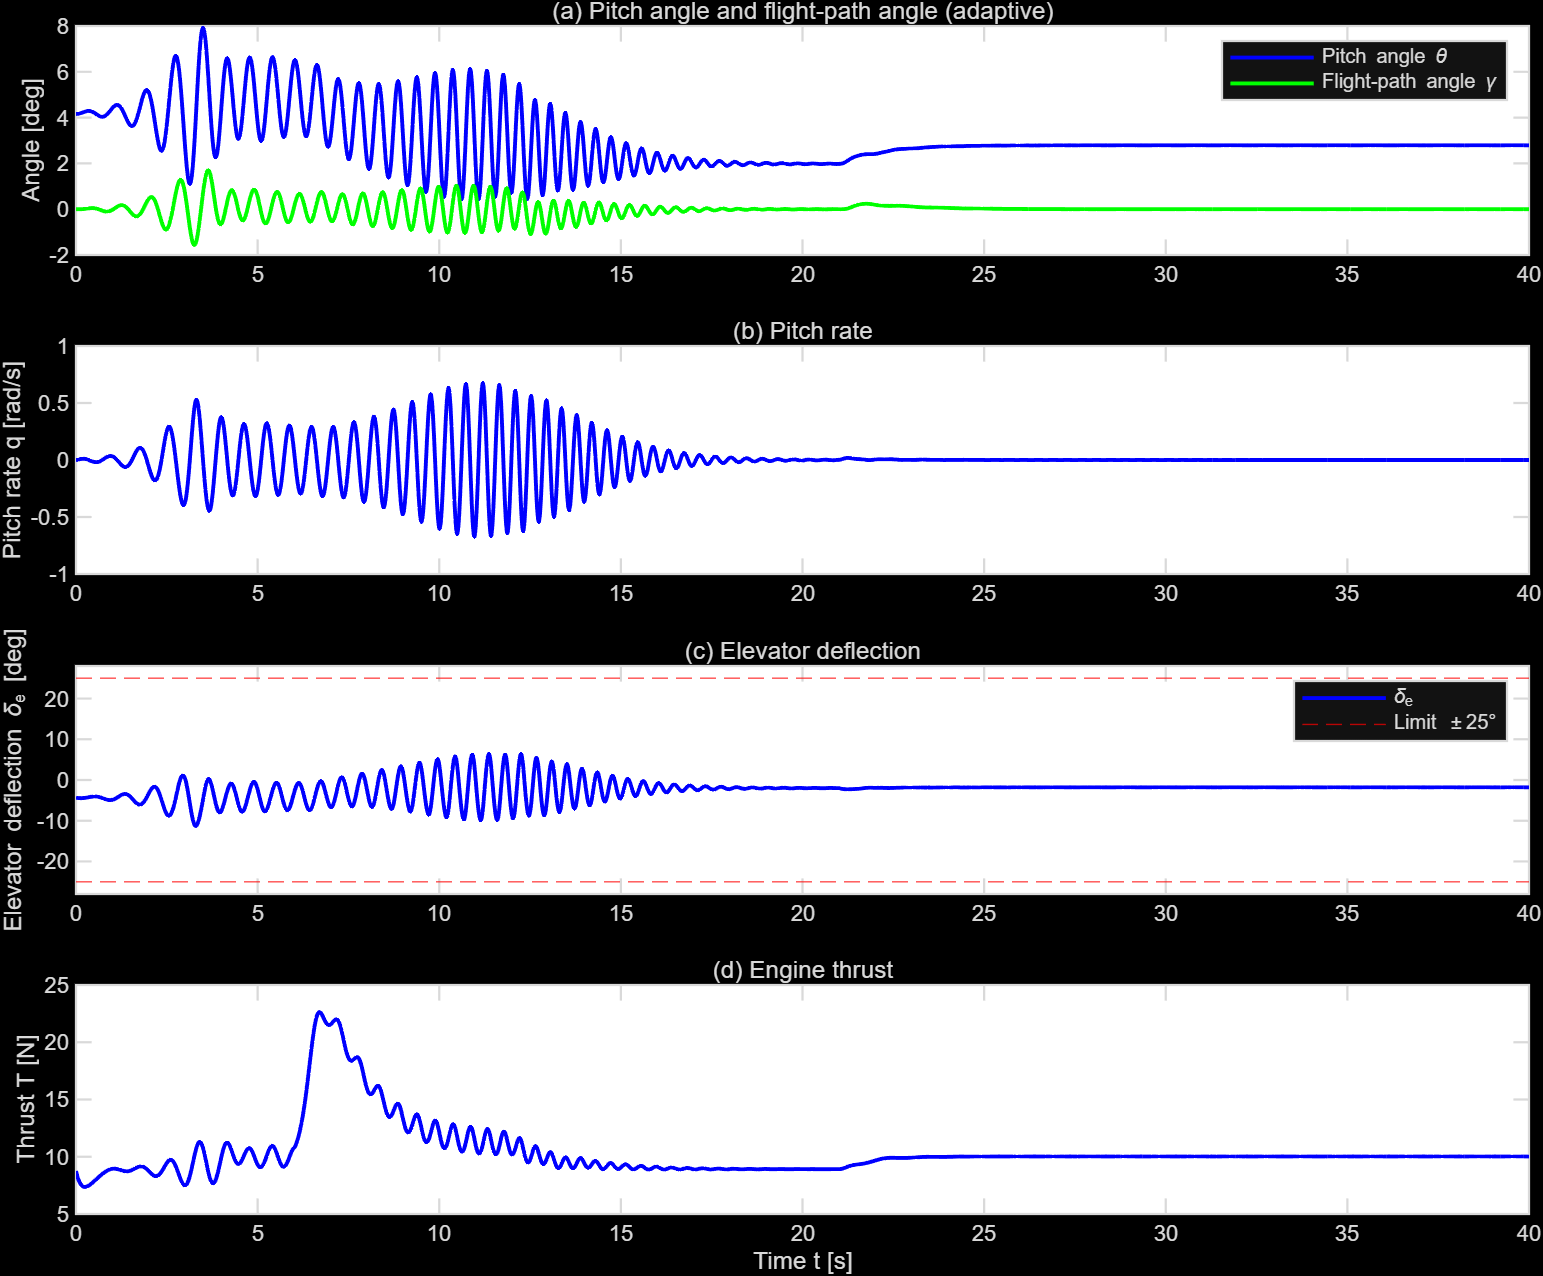
\includegraphics[width=1.00\linewidth]{fig5_states}
\vspace{2pt}
\caption{Pitch angle, flight-path angle, pitch rate, elevator and thrust under adaptive control.}
\label{fig:states}
\end{figure}

Fig. 7 shows the adaptive signals. The moment-channel output $u_M$ adjusts continuously during the height manoeuvre to compensate the ground-effect mismatch and the RAM moment; the weight norm remains bounded by the projection operator and settles at $\|W_1\| \approx 0.044$ under steady conditions. The drag-channel output $u_D$ compensates a drag mismatch of about 1.6 N, keeping the airspeed RMS error at only 9.9000 m/s.

\begin{figure}[!t]
\centering
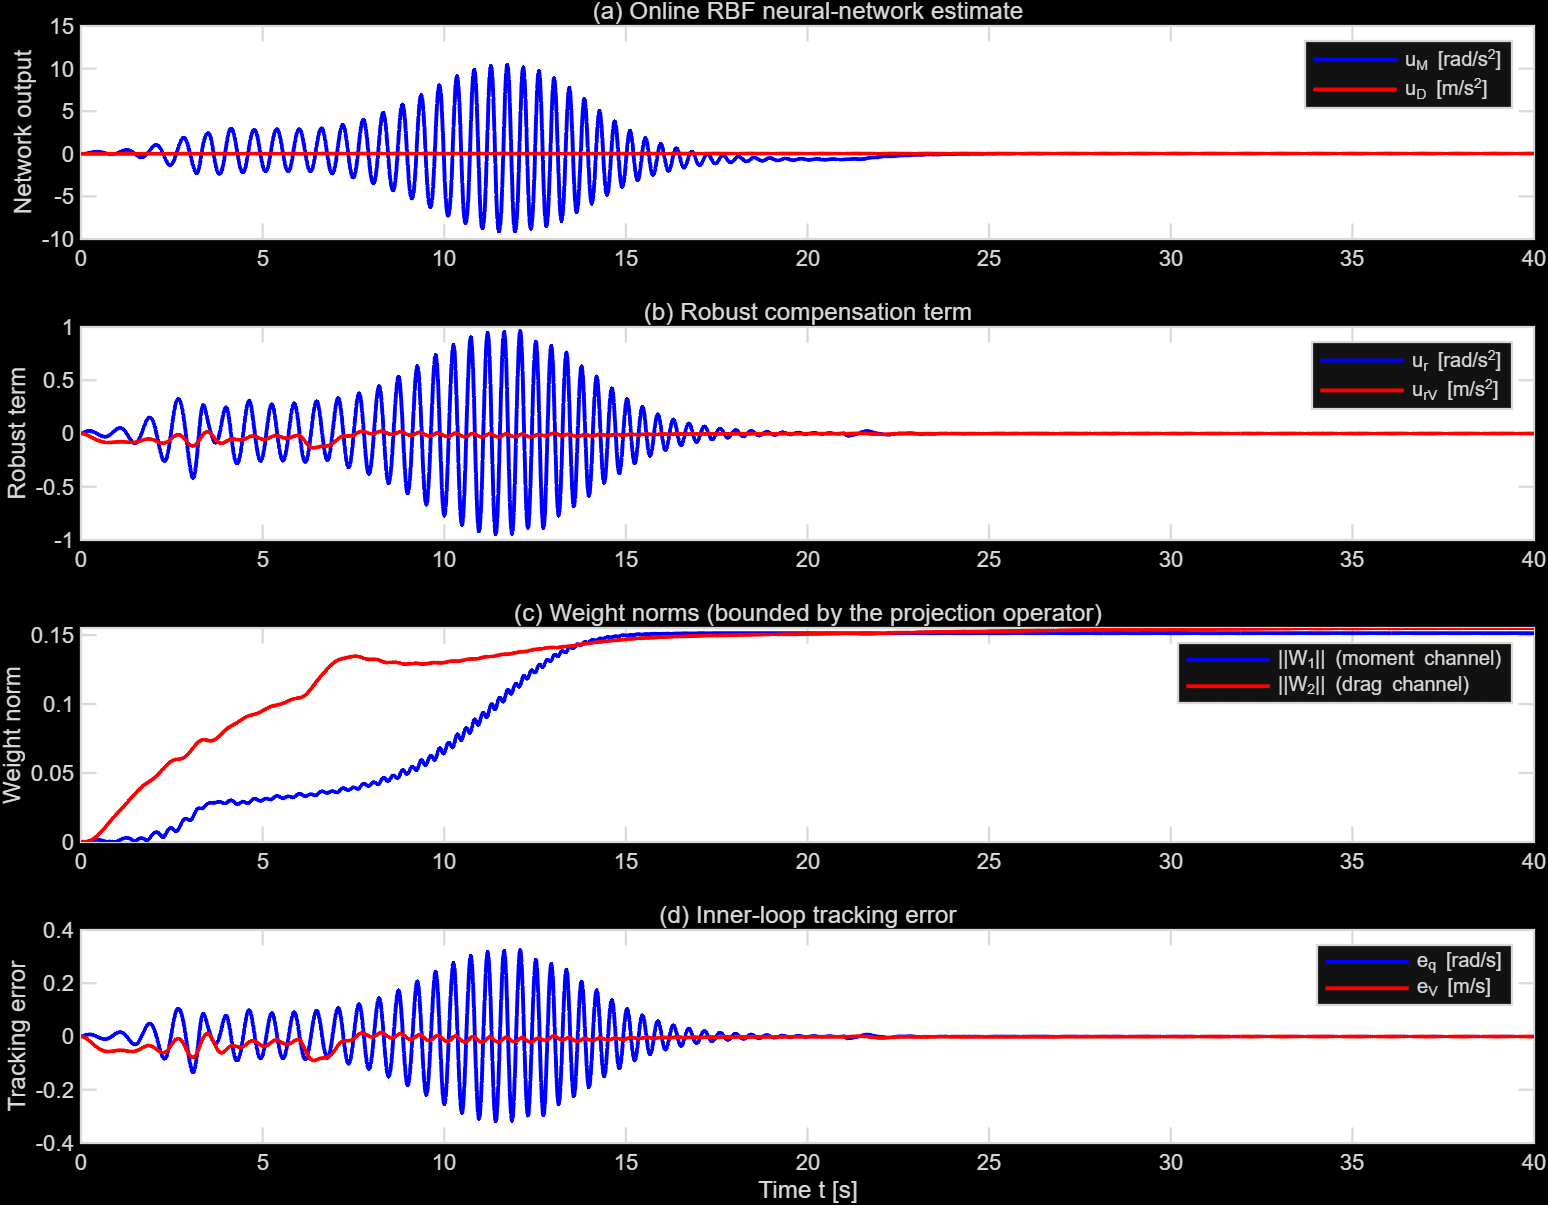
\includegraphics[width=1.00\linewidth]{fig6_adaptive}
\vspace{2pt}
\caption{RBF network outputs, robust terms, weight norms and tracking errors versus time.}
\label{fig:adaptive}
\end{figure}

\subsection{Parameter Perturbation}
7 extreme perturbation cases are added to the nominal plant, covering mass, ground-effect strength, drag coefficient, downwash gradient and lift-curve slope. In all 8 cases the vehicle does not touch the ground and the height RMS error stays between 0.0048 and 0.0425 m.

\begin{table*}[!t]
\centering
\caption{Performance under parameter perturbation (RBF adaptive controller)}
\label{tab:pert}
\footnotesize
\setlength{\tabcolsep}{4pt}
\begin{adjustbox}{max width=\textwidth}
\wigmeasure{pert}{%
\begin{tabular}{lccccc}
\toprule
Case & $h_{rms}$ / m & Peak height error / m & $h_{\min}$ / m & Peak $\delta_e$ / deg & Safe \\
\midrule
Nominal plant & 0.0100 & 0.0420 & 0.1000 & 9.9 & yes \\
Mass $m$ x1.25, $I_{yy}$ x1.26 & 0.0069 & 0.0282 & 0.0998 & 8.4 & yes \\
Mass $m$ x0.85, $I_{yy}$ x0.826 & 0.0425 & 0.1441 & 0.0892 & 13.7 & yes \\
GE shape parameter $A$ x0.312 (stronger GE) & 0.0077 & 0.0361 & 0.0995 & 9.9 & yes \\
GE shape parameter $A$ x1.404 (weaker GE) & 0.0048 & 0.0162 & 0.0933 & 5.2 & yes \\
Parasite drag $C_{D0}/C_{D0t}$ x1.80 (+80\%) & 0.0100 & 0.0414 & 0.1000 & 10.1 & yes \\
Downwash gradient $\varepsilon_\alpha$ x1.94 (+94\%) & 0.0105 & 0.0544 & 0.1000 & 11.6 & yes \\
Lift slope $a_0$ x0.881, tail efficiency $\eta_t$ x0.842 & 0.0107 & 0.0443 & 0.0998 & 10.9 & yes \\
\bottomrule
\end{tabular}}
\end{adjustbox}
\end{table*}

\begin{figure}[!t]
\centering
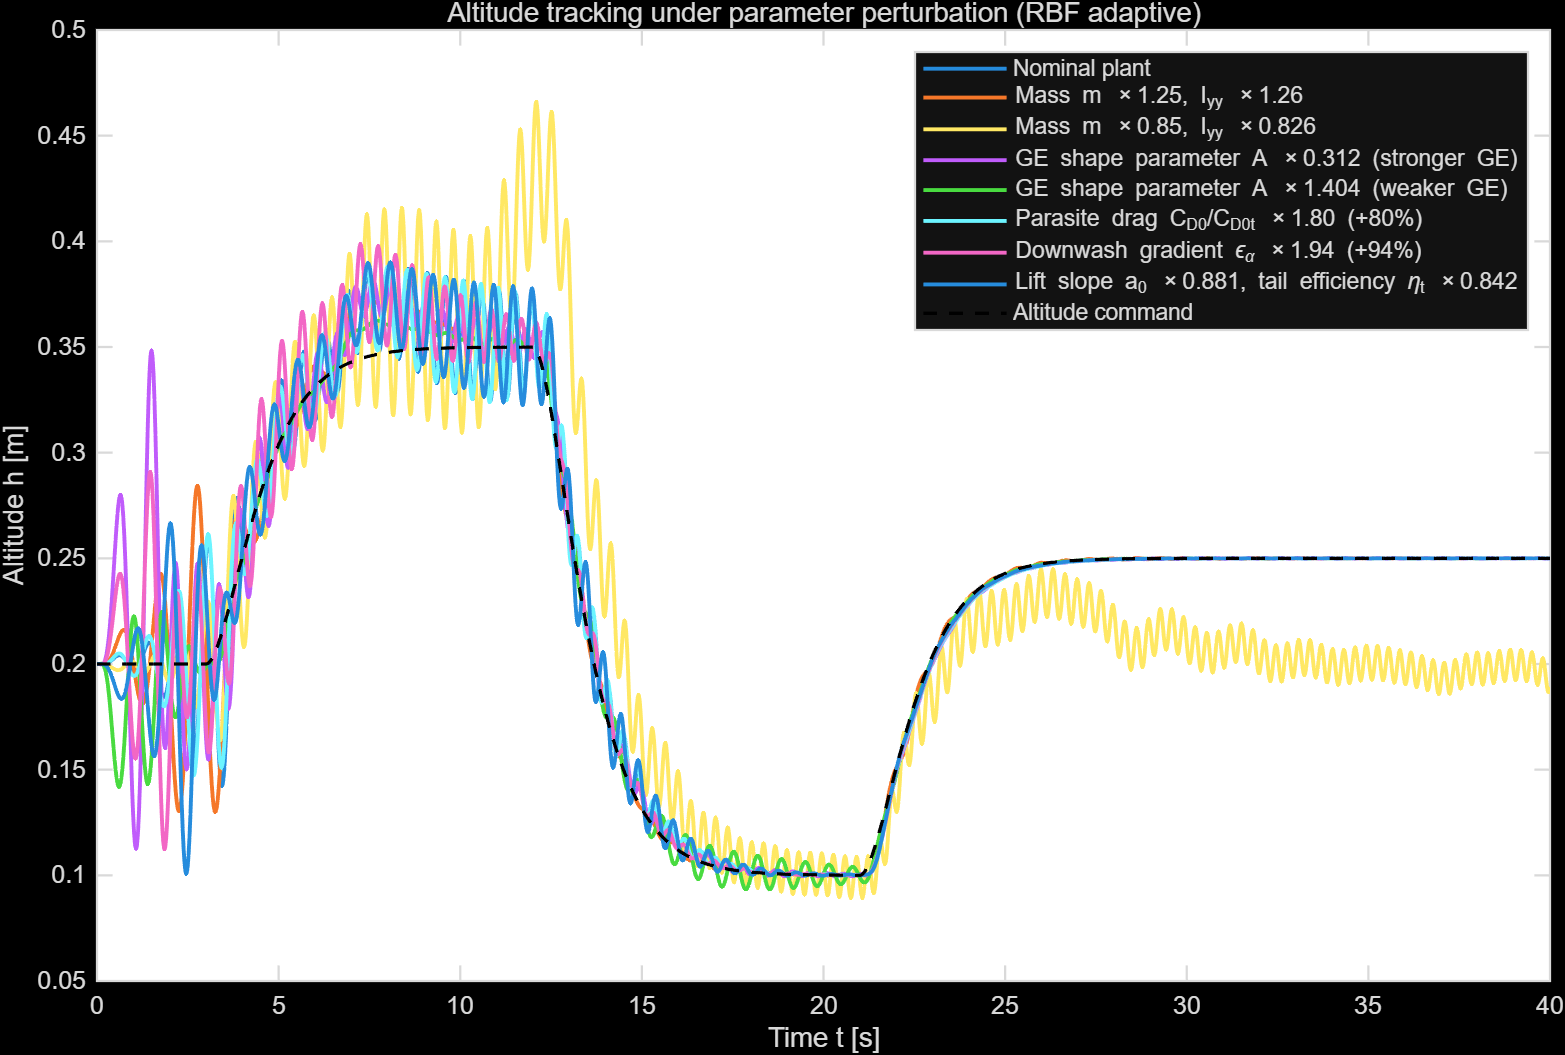
\includegraphics[width=1.00\linewidth]{fig7_perturbation}
\vspace{2pt}
\caption{Height tracking under parameter perturbation.}
\label{fig:pert}
\end{figure}

\subsection{Atmospheric Disturbance}
Discrete 1-cos gusts and Dryden continuous turbulence are simulated; the results are given in Table X.

\begin{table*}[!t]
\centering
\caption{Performance under atmospheric disturbance}
\label{tab:gust}
\footnotesize
\setlength{\tabcolsep}{4pt}
\begin{adjustbox}{max width=\textwidth}
\wigmeasure{gust}{%
\begin{tabular}{lccccc}
\toprule
Disturbance & Adaptive $h_{rms}$ / m & Adaptive $h_{\min}$ / m & Safe & No adaptation $h_{rms}$ / m & Safe \\
\midrule
Discrete 1-cos gust, 1.5 m/s (moderate) & 0.0115 & 0.1000 & yes & 0.2424 & no \\
Discrete 1-cos gust, 3.0 m/s (severe) & 0.1109 & 0.0000 & no & 0.2425 & no \\
Dryden continuous turbulence, $\sigma$ = 1.5 m/s & 0.0098 & 0.0970 & yes & 0.1892 & no \\
\bottomrule
\end{tabular}}
\end{adjustbox}
\end{table*}

In a moderate gust (1.5 m/s) and in continuous turbulence ($\sigma = 1.5$ m/s) the adaptive controller gives height RMS errors of 0.0115 m and 0.0098 m respectively, without ground contact, whereas switching the adaptation off causes ground contact in both cases.

It must be stated honestly that in a severe gust ($W_g = 3.0$ m/s) the adaptive controller also touches the ground ($h_{rms} = 0.1109$ m). The reason is that a 3.0 m/s vertical gust produces an equivalent angle-of-attack step of about 9.46 deg for this vehicle, corresponding to a lift disturbance of about 141.7\% of weight, which exceeds the physical capability of the actuators and the available height margin. This result shows that the ground-effect flight envelope of the present configuration is relatively sensitive to vertical gusts, and that operational weather limits or a larger height margin are required in practice.

\begin{figure}[!t]
\centering
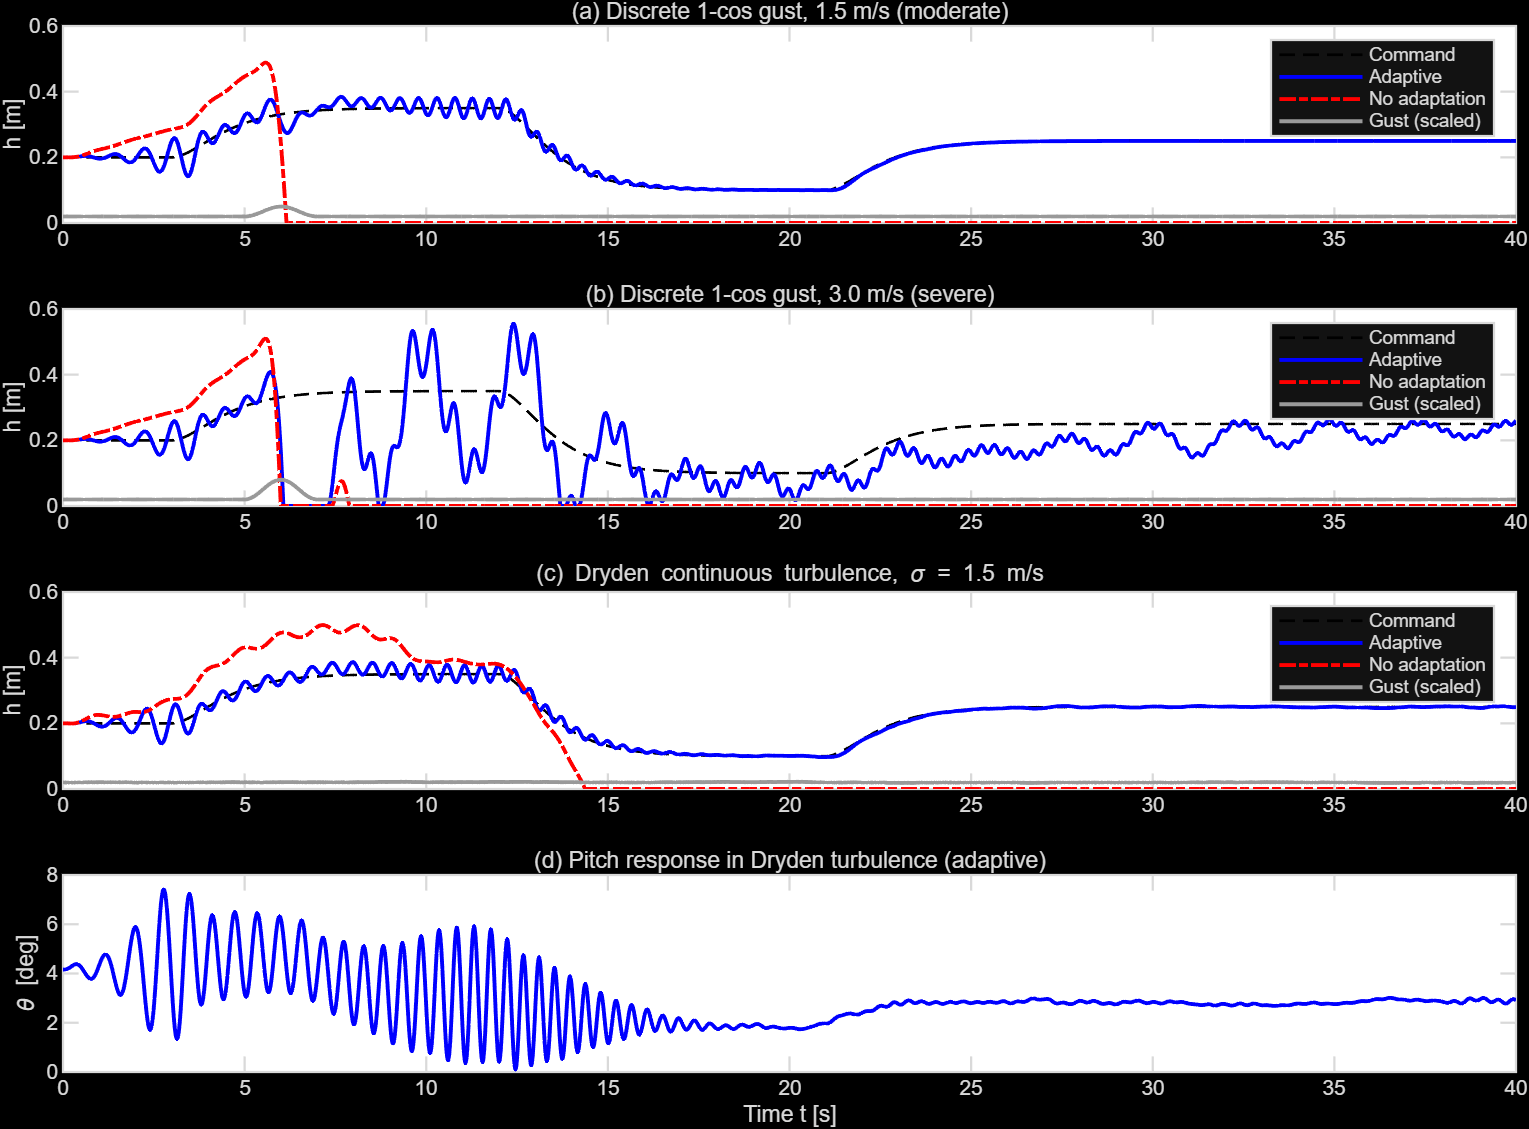
\includegraphics[width=1.00\linewidth]{fig8_gust}
\vspace{2pt}
\caption{Height response under gust and turbulence.}
\label{fig:gust}
\end{figure}

\subsection{Extreme Low-Altitude Flight and Measurement Noise}
The controller is assessed in the most demanding case: the height command drops to 0.06 m ($h/c = 0.15$, deep inside the ground-effect region) while measurement noise is added (airspeed 0.15 m/s, angle of attack 0.15 deg, pitch rate 0.3 deg/s, height 0.01 m) and actuator limits are active. The adaptive controller gives a height RMS error of 0.0082 m and a minimum height above ground of 0.0561 m with no ground contact and a peak elevator deflection of only 8.8 deg; with the adaptation switched off the height RMS error rises to 0.1295 m and the vehicle touches down.

\begin{figure}[!t]
\centering
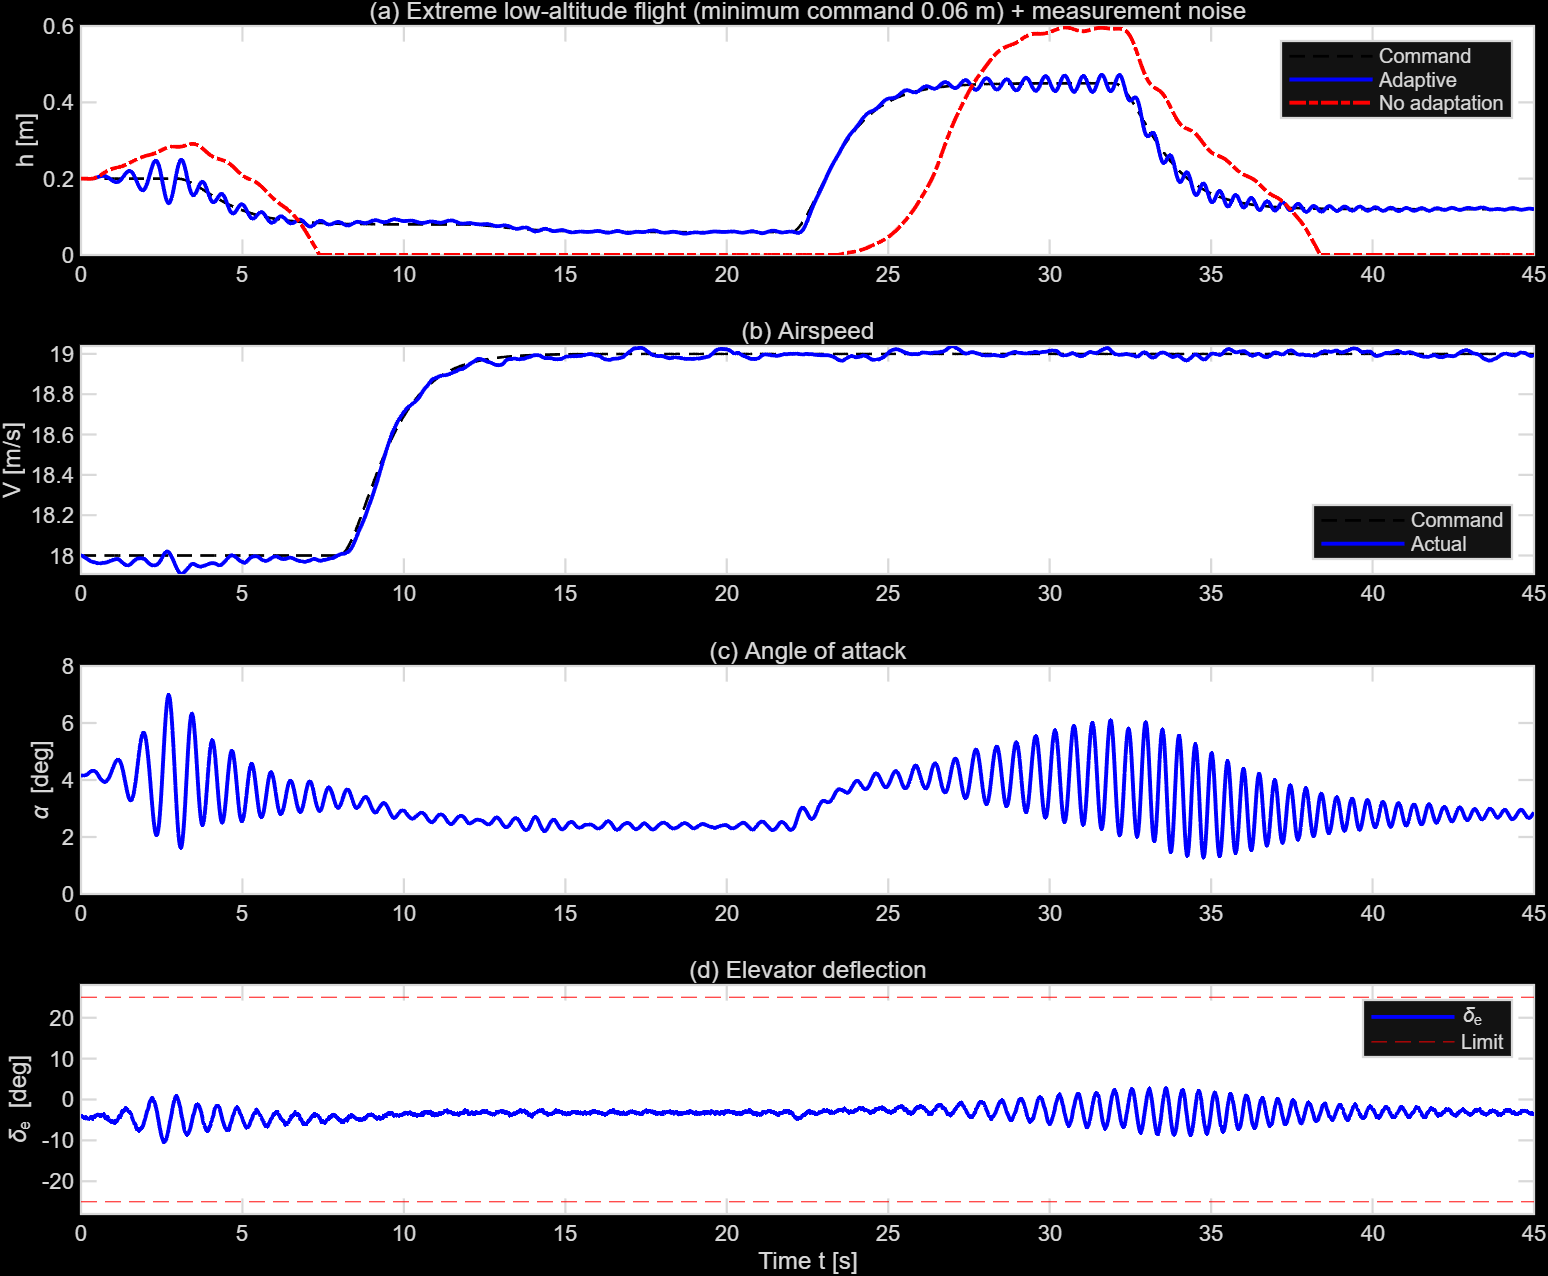
\includegraphics[width=1.00\linewidth]{fig9_lowalt}
\vspace{2pt}
\caption{Extreme low-altitude flight (minimum command 0.06 m) with measurement noise.}
\label{fig:lowalt}
\end{figure}

\subsection{Monte-Carlo Robustness Statistics}
60 samples are drawn independently and uniformly within the ranges: mass $\pm 25$\%, inertia $\pm 25$\%, parasite drag $\pm 40$\%, lift-curve slope $\pm 10$\%, pitch-moment coefficient $\pm 30$\%, ground-effect strength parameter $\pm 60$\%, downwash gradient $\pm 40$\%, tail efficiency $\pm 15$\%, initial height offset $\pm 0.03$ m and initial speed offset $\pm 1.0$ m/s.

\begin{table}[!t]
\centering
\caption{Monte-Carlo statistics (60 random parameter samples)}
\label{tab:mc}
\footnotesize
\setlength{\tabcolsep}{4pt}
\begin{adjustbox}{max width=\columnwidth}
\wigmeasure{mc}{%
\begin{tabular}{lccccc}
\toprule
Metric & Mean & Std & Median & 95th pct & Max \\
\midrule
Height RMS error / m & 0.04566 & 0.07107 & 0.01040 & 0.22652 & 0.28088 \\
Peak height error / m & 0.13986 & 0.21412 & 0.02946 & 0.66292 & 0.82895 \\
Minimum height above ground / m & 0.07757 & 0.03516 & 0.09183 & 0.10006 & 0.15310 \\
Peak airspeed error / (m/s) & 0.11882 & 0.10164 & 0.08286 & 0.35374 & 0.53118 \\
\bottomrule
\end{tabular}}
\end{adjustbox}
\end{table}

The pass rate (no ground contact and convergent) of the adaptive controller is 52/60 = 86.7\%, against 24/60 = 40.0\% without adaptation; the median height RMS error falls from 0.22322 m to 0.01040 m, an improvement of 21.5 times. The final weight norms have mean 0.282 and maximum 0.746 for $\|W_1\|$, both far below the projection bound $W_{\max} = 12.0$, confirming that the adaptation law operates well inside the safe region.

\begin{figure}[!t]
\centering
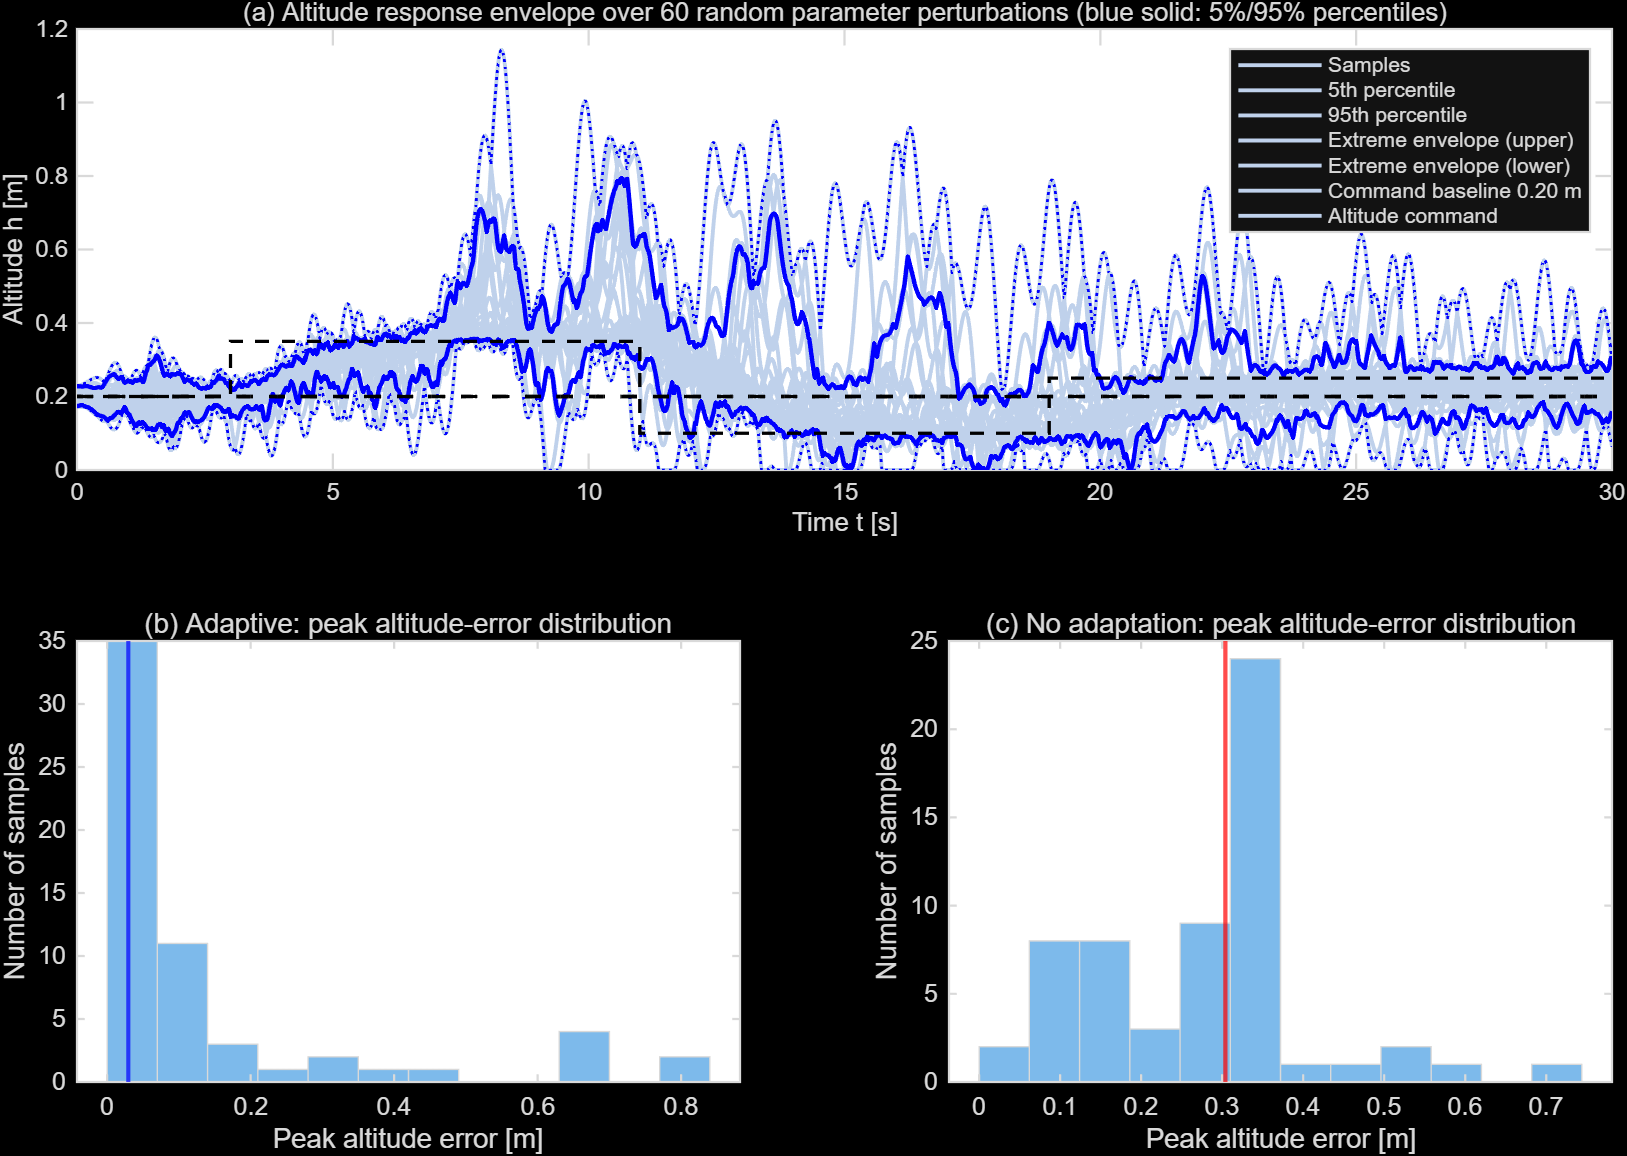
\includegraphics[width=1.00\linewidth]{fig10_montecarlo}
\vspace{2pt}
\caption{Monte-Carlo height envelope and distribution of the peak height error.}
\label{fig:mc}
\end{figure}

\subsection{Simulink Cross-Validation}
The same case is simulated both with a Simulink model and with the pure MATLAB script. Both share the same plant and controller code; only the integrator and the scheduling are provided by Simulink. The comparison must respect consistent signal definitions: the Simulink $u$ channel records the controller \textbf{command}, whereas the script records the actuator \textbf{state}, and the two differ by a first-order lag of $\tau_e = 0.05$ s (up to about $6^{\circ}$ under the 120 deg/s rate limit). Table XII therefore reports both state-versus-state and command-versus-command comparisons.

\begin{table}[!t]
\centering
\caption{Simulink model versus pure MATLAB script}
\label{tab:simtab}
\footnotesize
\setlength{\tabcolsep}{4pt}
\begin{adjustbox}{max width=\columnwidth}
\wigmeasure{simtab}{%
\begin{tabular}{lccc}
\toprule
Metric & Simulink & MATLAB script & Deviation \\
\midrule
Height RMS error / m & 0.009959 & 0.009977 & 1.74e-05 \\
Peak height error / m & 0.042039 & 0.041998 & 4.13e-05 \\
Minimum height / m & 0.100019 & 0.100020 & 1.56e-06 \\
Airspeed RMS error / (m/s) & 0.012358 & 0.012602 & 2.44e-04 \\
Peak elevator (state) / deg & 11.2907 & 11.2933 & 2.63e-03 \\
Peak elevator (command) / deg & 11.9204 & 11.9232 & 2.83e-03 \\
\bottomrule
\end{tabular}}
\end{adjustbox}
\end{table}

The largest trajectory deviations (state versus state) are 1.279e-03 m in height, 4.386e-03 m/s in airspeed and 2.667e-01 deg in elevator deflection; the largest command deviation (command versus command) is 3.409e-01 deg. All are at the level of sampling and interpolation error, showing that the Simulink model and the script simulation are numerically equivalent and that the model can serve as a basis for hardware-in-the-loop testing and code generation.

\begin{figure}[!t]
\centering
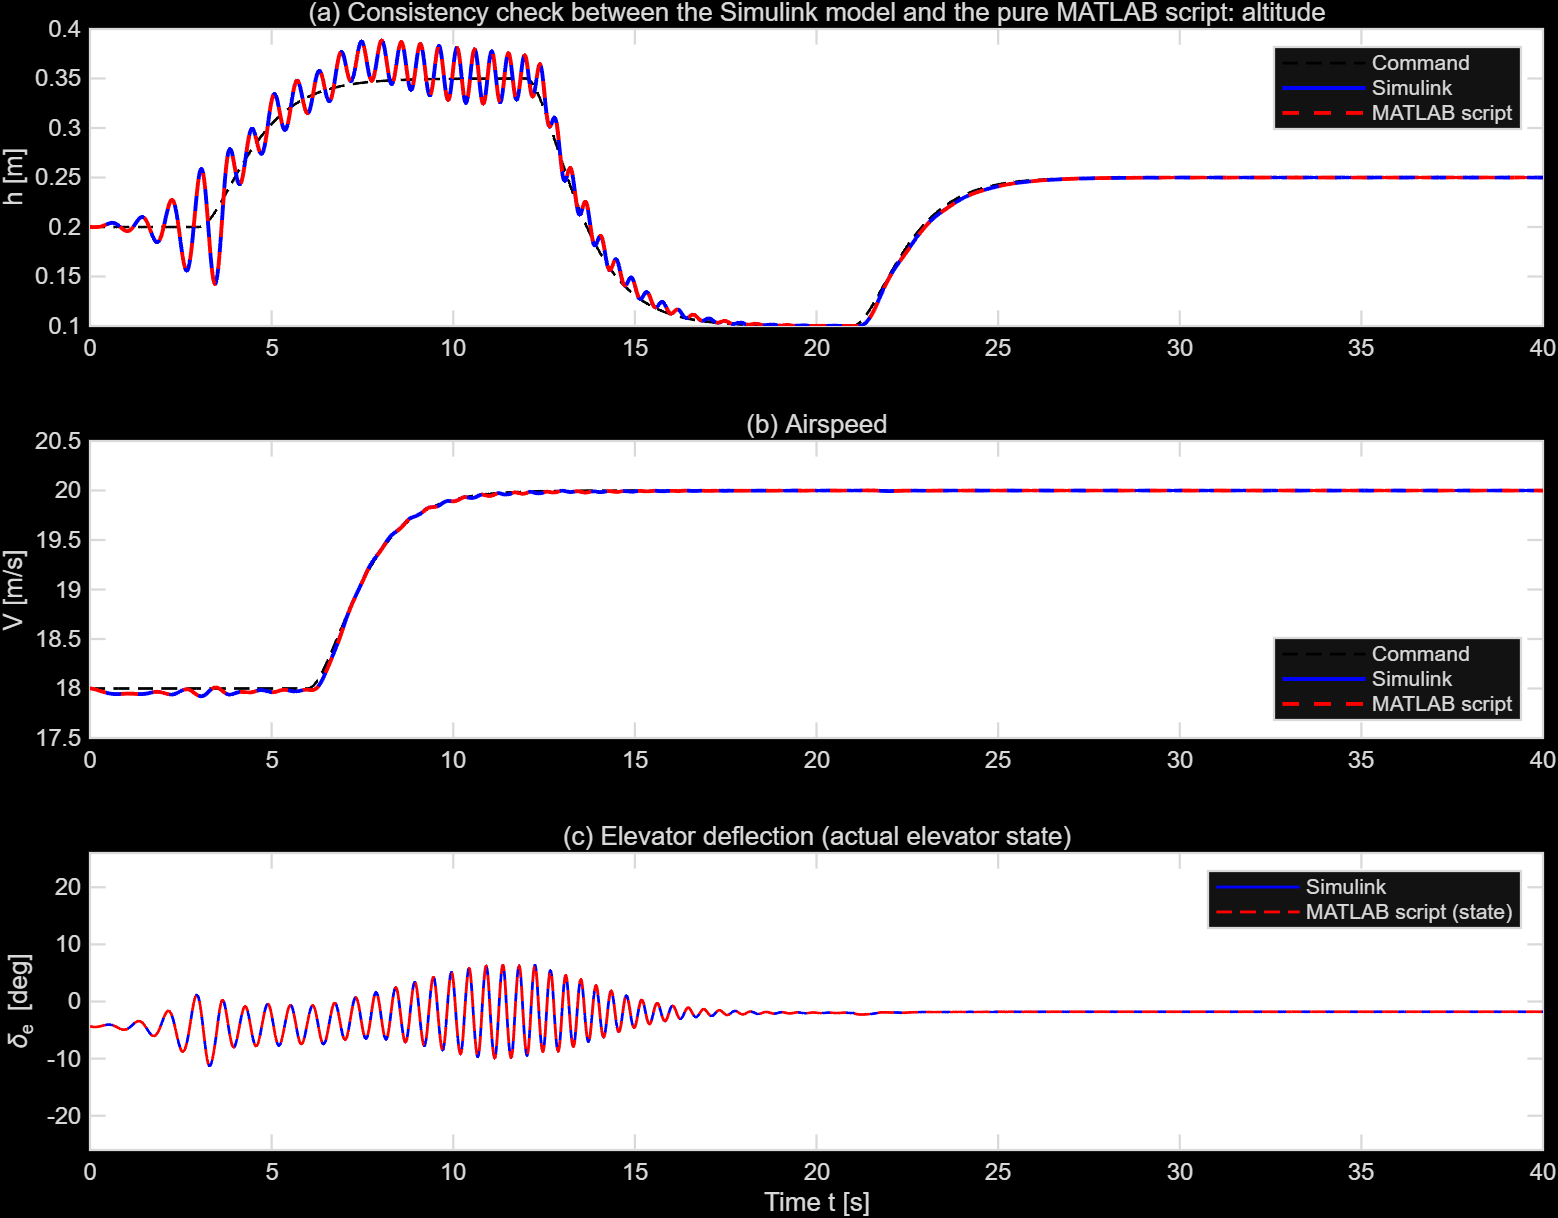
\includegraphics[width=1.00\linewidth]{fig11_simulink}
\vspace{2pt}
\caption{Consistency check between the Simulink model and the pure MATLAB script.}
\label{fig:simulink}
\end{figure}

\section{Conclusions}
This paper has studied the mechanism of ground-effect height instability and the design of an RBF neural-network adaptive longitudinal controller for a small WIG UAV. The main conclusions are as follows.

\begin{enumerate}
  \item A seventh-order nonlinear longitudinal model with ground-effect correction was established. Over $h/b = 0.02$ to $0.5$ the ground-effect factor reproduces the trends of published wind-tunnel and CFD data: at $h = 0.05$ m the induced drag falls to 5.1\% of its free-air value and the lift-curve slope rises by 34.3\%, while at $h = 0.50$ m the lift-curve slope is still 11.7\% higher.
  \item The component-wise decomposition of $\partial M/\partial h$ revealed the height instability mechanism quantitatively: over the whole envelope $\partial M/\partial h = +1.06$ to +14.90 N$\cdot$m/m, positive everywhere, of which the tail downwash term contributes +15.78 N$\cdot$m/m (the dominant destabilising term), the wing term -2.30 N$\cdot$m/m (stabilising), and the RAM and lift-nonlinearity terms about +0.66 and +0.25 N$\cdot$m/m respectively (destabilising). The four terms sum to the numerical total to within 2.4e-12.
  \item The phugoid-height coupled mode instability was shown to originate entirely from the ground effect: with ground effect the real part is +0.1434 to +0.4875 1/s and the lowest damping ratio is -0.927, whereas switching the ground effect off returns the mode to neutral stability (real part -0.0275 to +0.0002 1/s).
  \item A three-loop controller, comprising an altitude outer loop, a dynamic-surface attitude inner loop and an airspeed loop, was designed, with RBF networks and tanh robust terms in the moment and drag channels. Closed-loop UUB was proved by a Lyapunov argument with an explicit residual bound. Using the kinematic identity $\theta_d = \gamma_c + \alpha$, the lift-channel error is compensated automatically by angle-of-attack feedback, removing an entire network.
  \item The discrete-time stability criterion $T_s\Gamma_i\|\phi_i\|^2 < k_i$ was derived, which explains why the moment-channel adaptation gain (0.005) is three orders of magnitude smaller than the drag-channel gain (3.0): the dimensional factors of the two regression vectors differ by about 795.
  \item Simulations showed that, with significant ground-effect mismatch, RAM effect and lift nonlinearity, the adaptive controller reduces the height RMS error from 0.1938 m to 0.0100 m (a factor of 19.4) and raises the Monte-Carlo pass rate from 40.0\% to 86.7\%, while maintaining safe flight at 0.06 m, under measurement noise and in moderate gusts. With the final gains the largest sampled closed-loop pole modulus is $\max|z| = 0.99942 < 1$.
\end{enumerate}

\subsection{Limitations and Future Work}
\begin{itemize}
  \item The aerodynamic model is quasi-steady and linear and neglects unsteady ground-effect hysteresis and high-angle-of-attack separation; CFD studies of pitching oscillation and rapid height variation are recommended to calibrate the dynamic derivatives and to test the validity of the quasi-steady assumption.
  \item The ground-effect parameters were calibrated to the trends of published data rather than to this specific configuration. Once CFD calibration is available the values can be written into the nominal model, reducing both the mismatch and the adaptation burden.
  \item In a severe vertical gust ($W_g = 3.0$ m/s) the controller still touches down, showing that the envelope of this configuration is sensitive to vertical gusts; gust alleviation (for example direct-lift control) and trajectory planning are possible remedies.
  \item Only the longitudinal channel is considered; lateral-directional and trajectory tracking remain for future work, for which a decoupled adaptive design can be extended.
  \item The robust boundary-layer thicknesses and adaptation gains are still tuned from nonlinear closed-loop indices; a more systematic design could use $\mu$-synthesis or an $\mathcal{L}_1$ adaptive framework.
\end{itemize}

\section{Appendix: Controller Tuning Parameters}
\begin{table}[!t]
\centering
\caption{Final controller tuning parameters}
\label{tab:tuning}
\footnotesize
\setlength{\tabcolsep}{4pt}
\begin{adjustbox}{max width=\columnwidth}
\wigmeasure{tuning}{%
\begin{tabular}{lcclcc}
\toprule
Parameter & Symbol & Value & Parameter & Symbol & Value \\
\midrule
Altitude loop gain & $k_h$ & 2.00 1/s & Pitch loop gain & $k_\theta$ & 3.20 1/s \\
Height-rate damping & $k_{hd}$ & 0.80 & Pitch-rate gain & $k_q$ & 6.00 1/s \\
Flight-path filter & $\tau_g$ & 0.010 s & Pitch command filter & $\tau_\theta$ & 0.100 s \\
Rate command filter & $\tau_q$ & 0.010 s & Airspeed loop gain & $k_V$ & 1.53 1/s \\
Airspeed integral gain & $k_{IV}$ & 0.42 1/s$^2$ & Moment channel gain & $\Gamma_1$ & 0.005 \\
Drag channel gain & $\Gamma_2$ & 3.0 & $e$-modification & $\nu_e$ & 0.50 \\
Moment robust gain & $\eta_r$ & 2.50 rad/s$^2$ & Moment boundary layer & $\Phi_r$ & 0.80 rad/s \\
Speed robust gain & $\eta_V$ & 1.50 m/s$^2$ & Speed boundary layer & $\Phi_V$ & 1.00 m/s \\
Weight projection bound & $W_{\max}$ & 12.0 & Pitch command limit & $\theta_{\max}$ & $20^{\circ}$ \\
Flight-path limit & $\gamma_{\max}$ & $12^{\circ}$ & RBF nodes & $N_1 / N_2$ & 75 / 64 \\
\bottomrule
\end{tabular}}
\end{adjustbox}
\end{table}

\section{References}
\begin{thebibliography}{99}
\bibitem{r1} K. V. Rozhdestvensky, "Wing-in-ground effect vehicles," Progress in Aerospace Sciences, vol. 42, no. 3, pp. 211-283, 2006, doi: 10.1016/j.paerosci.2006.10.001.
\bibitem{r2} A. Nebylov and V. Nebylov, "Wing-in-ground effect vehicles flight automatic control systems development problems," Applied Mechanics and Materials, vol. 629, pp. 370-375, 2014, doi: 10.4028/www.scientific.net/AMM.629.370.
\bibitem{r3} W. Yang, Z. Yang, and M. Collu, "Longitudinal static stability requirements for wing in ground effect vehicle," International Journal of Naval Architecture and Ocean Engineering, vol. 7, no. 2, pp. 259-269, 2015, doi: 10.1515/ijnaoe-2015-0018.
\bibitem{r4} J. Lee, "Computational analysis of static height stability and aerodynamics of vehicles with a fuselage, wing and tail in ground effect," Ocean Engineering, vol. 168, pp. 12-22, 2018, doi: 10.1016/j.oceaneng.2018.08.051.
\bibitem{r5} G. Kocak and M. M. Yavuz, "Effect of ground on aerodynamics and longitudinal static stability of a non-slender delta wing," Aerospace Science and Technology, vol. 130, art. no. 107929, 2022, doi: 10.1016/j.ast.2022.107929.
\bibitem{r6} P. E. Kumar, "Some stability problems of ground effect wing vehicles in forward motion," Aeronautical Quarterly, vol. 23, no. 1, pp. 41-52, 1972, doi: 10.1017/S0001925900006302.
\bibitem{r7} R. M. Sanner and J.-J. E. Slotine, "Gaussian networks for direct adaptive control," IEEE Transactions on Neural Networks, vol. 3, no. 6, pp. 837-863, 1992, doi: 10.1109/72.165588.
\bibitem{r8} M. M. Polycarpou, "Stable adaptive neural control scheme for nonlinear systems," IEEE Transactions on Automatic Control, vol. 41, no. 3, pp. 447-451, 1996, doi: 10.1109/9.486648.
\bibitem{r9} M. M. Polycarpou and P. A. Ioannou, "A robust adaptive nonlinear control design," Automatica, vol. 32, no. 3, pp. 423-427, 1996, doi: 10.1016/0005-1098(95)00147-6.
\bibitem{r10} P. A. Ioannou and J. Sun, Robust Adaptive Control. Englewood Cliffs, NJ, USA: Prentice Hall, 1996, ISBN 0-13-439100-4.
\bibitem{r11} D. Swaroop, J. K. Hedrick, P. P. Yip, and J. C. Gerdes, "Dynamic surface control for a class of nonlinear systems," IEEE Transactions on Automatic Control, vol. 45, no. 10, pp. 1893-1899, 2000, doi: 10.1109/TAC.2000.880994.
\bibitem{r12} J. A. Farrell, M. Polycarpou, M. Sharma, and W. Dong, "Command filtered backstepping," IEEE Transactions on Automatic Control, vol. 54, no. 6, pp. 1391-1395, 2009, doi: 10.1109/TAC.2009.2015562.
\bibitem{r13} P. P. Yip and J. K. Hedrick, "Adaptive dynamic surface control: a simplified algorithm for adaptive backstepping control of nonlinear systems," International Journal of Control, vol. 71, no. 5, pp. 959-979, 1998, doi: 10.1080/002071798221650.
\bibitem{r14} S. S. Ge and C. Wang, "Adaptive NN control of uncertain nonlinear pure-feedback systems," Automatica, vol. 38, no. 4, pp. 671-682, 2002, doi: 10.1016/S0005-1098(01)00254-0.
\bibitem{r15} C. E. Rohrs, L. Valavani, M. Athans, and G. Stein, "Robustness of continuous-time adaptive control algorithms in the presence of unmodeled dynamics," IEEE Transactions on Automatic Control, vol. 30, no. 9, pp. 881-889, 1985, doi: 10.1109/TAC.1985.1104070.
\bibitem{r16} S. Akhtar and D. S. Bernstein, "Lyapunov-stable discrete-time model reference adaptive control," in Proc. American Control Conference, Portland, OR, USA, 2005, pp. 3174-3179, doi: 10.1109/ACC.2005.1470460.
\bibitem{r17} F.-C. Chen and H. K. Khalil, "Adaptive control of a class of nonlinear discrete-time systems using neural networks," IEEE Transactions on Automatic Control, vol. 40, no. 5, pp. 791-801, 1995, doi: 10.1109/9.384214.
\bibitem{r18} R. Staufenbiel, "Some nonlinear effects in stability and control of wing-in-ground effect vehicles," Journal of Aircraft, vol. 15, no. 8, pp. 541-544, 1978, doi: 10.2514/3.58404.
\bibitem{r19} J. Gera, "Stability and control of wing-in-ground effect vehicles or wingships," in 33rd Aerospace Sciences Meeting and Exhibit, Reno, NV, USA: AIAA, 1995, doi: 10.2514/6.1995-339.
\bibitem{r20} A. Fevralskikh, "A development of longitudinal static stability analysis method of a wing-in-ground effect vehicle in cruise during the design process," Ocean Engineering, vol. 243, art. no. 110187, 2022, doi: 10.1016/j.oceaneng.2021.110187.
\bibitem{r21} Y. Zhang, S. Chen, J. Xu, and J. Li, "An improved approach for aerodynamic optimization considering WIG effect and height static stability," Aerospace Science and Technology, vol. 160, art. no. 110071, 2025, doi: 10.1016/j.ast.2025.110071.
\bibitem{r22} O. Li and L. Deng, "Dynamic surface adaptive control for air-breathing hypersonic vehicles based on RBF neural networks," Aerospace, vol. 12, no. 11, art. no. 984, 2025, doi: 10.3390/aerospace12110984.
\bibitem{r23} T. Le and L. Wang, "Research on longitudinal stability and aerodynamic configuration characteristics of ground-effect aircraft," Flight Dynamics, vol. 25, no. 3, pp. 5-8, 2007 (in Chinese).
\bibitem{r24} Y. Li, W. Yang, and Z. Yang, "Numerical study on longitudinal static stability of a canard ground-effect vehicle," Flight Dynamics, vol. 28, no. 1, pp. 9-12, 2010 (in Chinese).
\bibitem{r25} Y. Luo and H. Fan, "Research on longitudinal stability and stability augmentation system of ground effect aircraft," Computer Measurement \& Control, vol. 30, no. 4, pp. 134-141, 2022 (in Chinese).
\bibitem{r26} Y. Huo, M. Mirmirani, P. Ioannou, and M. Kuipers, "Altitude and velocity tracking control for an airbreathing hypersonic cruise vehicle," in AIAA Guidance, Navigation, and Control Conference and Exhibit, Keystone, CO, USA: AIAA, 2006, doi: 10.2514/6.2006-6695.
\end{thebibliography}

\end{document}
